\documentclass[letterpaper,twocolumn]{article}

\usepackage{bigdelim}
\usepackage{graphicx}
\usepackage{makecell}
\usepackage{multirow}
\usepackage{pifont} % For checkmarks in tab:nat-matching.
\usepackage{titling}
\usepackage[hyphens]{url}
\usepackage[table]{xcolor}

% Better look for citations that include a section reference like \cite[\S 3]{foobar}.
\usepackage{cite}
\renewcommand{\citemid}{~}

% Load hyperref after other packages.
\usepackage[pdfa,hidelinks,pdfusetitle,pdfcreator={},pdfproducer={}]{hyperref}
\urlstyle{same}
\def\sectionautorefname{Section}
\def\subsectionautorefname{Section}

\usepackage{usenix-2020-09}

% Disable metadata for reproducible PDF.
% https://tex.stackexchange.com/a/313605
\usepackage{ifpdf}
\ifpdf
\pdfinfoomitdate=1
\pdftrailerid{}
\pdfsuppressptexinfo=-1
\fi

\hyphenation{Web-RTC}
\hyphenation{Web-Exten-sion}
\hyphenation{Java-Script}
\hyphenation{uProxy}
\hyphenation{off-line}
\hyphenation{mac-OS}

% Highlight the first usage or definition of a technical term.
% Like the firstterm element in DocBook: https://tdg.docbook.org/tdg/5.2/firstterm.html.
\newcommand{\firstterm}[1]{\textit{#1}}

\begin{document}

\date{}

\title{\Large\bf Snowflake, a censorship circumvention system\\using temporary WebRTC proxies}

% \author{%
% {\rm Cecylia Bocovich}%
% \and
% {\rm Arlo Breault}%
% \and
% {\rm David Fifield}%
% \and
% {\rm Serene}%
% \and
% {\rm Xiaokang Wang}%
% }
% \renewcommand{\maketitlehookc}{\centering\normalsize Authors are listed alphabetically.}

\maketitle

\begin{abstract}
Snowflake is a system for circumventing Internet censorship.
Its blocking resistance comes from
the use of numerous, ultra-light, temporary proxies (``snowflakes''),
which accept traffic from censored clients using peer-to-peer WebRTC protocols
and forward it to a centralized bridge,
which does the real work of directing traffic to its destination.
The temporary proxies are lightweight enough to be implemented in JavaScript,
in~a web page or browser extension,
making them vastly cheaper to set up than
a traditional proxy or VPN server.
The proxies do not need to have stable network addresses,
nor be continually online---even
the disappearance of an \mbox{in-use} proxy
does not mean the end of a circumvention session,
as its client will switch to another on the fly,
invisibly to upper network layers.

% Need anything about broker, centralization here?

Snowflake has been deployed with success
in Tor Browser and Orbot for several years.
It has been significant for circumvention
during high-profile network disruptions,
including in Russia in~2021 and Iran in~2022.
In this paper, we explain the composition of Snowflake's many parts,
give a history of deployment and attempts to block~it,
and reflect on implications for circumvention generally.
\end{abstract}

% General references:
%   https://keroserene.net/snowflake/technical/#history
%   https://www.bamsoftware.com/papers/thesis/#chap:snowflake

\section{Introduction}
\label{sec:intro}

Censorship circumvention systems---systems
to enable network communication
despite interference by a censor---may
be characterized on multiple axes.
Some systems imitate a common network protocol;
others try
not to look like any protocol in particular.
Some distribute connections over numerous proxy servers;
others concentrate on a single proxy
that is, for one reason or another, difficult for a censor to block.
What all circumvention systems have in common
is that they strive to increase the \emph{cost}
to the censor of blocking them---whether that cost be in
research and development, human resources, and hardware;
or in the inevitable overblocking that results
when a censor tries to selectively block
some connections but not others.
Snowflake, the subject of this paper,
is a circumvention system that
uses thousands of temporary proxies
and makes switching between them easy and fast.
On~the spectrum of imitation to randomization,
Snowflake falls on the side of imitation;
on the scale from diffuse to concentrated, it is diffuse.
What most sets Snowflake apart is that
it pushes the idea of distributed, disposable
proxies to an extreme:
its~proxies can run in a web browser
and censored clients communicate with them using WebRTC.

WebRTC is a suite of protocols
intended for real-time communication applications
in web browsers~\cite{rfc8825}.
Video and voice chat are typical examples
of WebRTC applications.
Snowflake exchanges WebRTC data formats
in the course of establishing a connection,
and uses WebRTC protocols for traversal of NAT (network address translation)
and communication between clients and proxies.
Crucially for Snowflake, WebRTC APIs
are available to JavaScript code in web browsers,
meaning it is possible to implement a proxy
in a web page or browser extension.
WebRTC is also usable outside a browser,
which is how we implement the Snowflake client program
and alternative, command line--based proxies.

As~is usual in circumvention research,
we assume a threat model in which
\firstterm{clients} reside in a network
controlled by a \firstterm{censor}.
The censor has the power to inspect and interfere with
traffic that crosses the border of its network;
typical real-world censor behaviors include
inspecting IP addresses and hostnames,
checking packet contents for keywords,
blocking IP addresses, and injecting false DNS responses
or TCP RST packets.
The client wants to communicate with some
\firstterm{destination} outside the censor's network,
possibly with the aid of third-party \firstterm{proxies}.
The censor is motivated to block the contents
of the client's communication, or even the destination itself.
The censor is aware of the possibility of circumvention,
and therefore seeks to block not only direct communication,
but also indirect communication by way of a proxy or circumvention system.
Circumvention is accomplished when the client
can reliably reach any proxy,
because a proxy, being outside the censor's control,
can then forward the client's communication to any destination.
(In Snowflake, we separate the roles of temporary \firstterm{proxies}
and a stable long-term \firstterm{bridge}, but the goal is the same.)
The censor is presumed to derive benefit
from permitting some forms of network access:
the censor cannot trivially ``win''
by shutting down all communication,
but must be selective in its blocking decisions
in order to optimize some objective of its own.
The art of censorship circumvention is
forcing the censor into a dilemma
of overblocking or underblocking,
by making circumvention traffic difficult to distinguish
from traffic that the censor prefers not to block.

Snowflake originates in two earlier projects:
flash proxy and uProxy.
% https://lists.torproject.org/pipermail/tor-dev/2016-January/010310.html "Snowflake is a webrtc pluggable transport inspired by flashproxy."
% https://keroserene.net/snowflake/technical/#1-introduction "It is inspired by and builds upon the previous work of Flashproxy. Snowflake is much like a hybrid of previous Pluggable Transports..."
Flash proxy~\cite{Fifield2012a}, like Snowflake, used a model
of untrusted, temporary JavaScript proxies in web browsers,
but the link between client and proxy used WebSocket
rather than WebRTC.
(WebSocket still finds use in Snowflake,
but on the proxy--bridge link,
not the client--proxy link.)
Flash proxy was deployed in Tor Browser
% 2013: https://blog.torproject.org/combined-flash-proxy-pyobfsproxy-browser-bundles
% 2016: "Remove Flashproxy from Tor Browser" https://bugs.torproject.org/17428#note_2203210
from 2013 to~2016,
but never saw much use,
probably because the reliance on WebSocket,
which lacks the built-in NAT traversal of WebRTC,
required client users to do their own port forwarding.
% https://gitlab.torproject.org/legacy/trac/-/wikis/doc/PluggableTransports/FlashProxy/Howto
WebRTC was then an emerging technology, and while
% "Investigate WebRTC for flash proxy NAT punching" https://bugs.torproject.org/5578
% flashproxy.pdf §5.2: "New technologies like WebRTC [24] may fill this need in the future, if they become sufficiently popular that flash proxies' use of them does not stand out as unusual."
it had been considered as a transport protocol for flash proxy,
we decided to start Snowflake as an independent project.
% https://serene.cx/snowflake/#note-flashproxy "...one could say that uProxy and flashproxy are the ancestors of snowflake."
uProxy~\cite{uproxy}, in one of its early incarnations,
% "in one of its earlier incarnations": uProxy pivoted from friend proxies to cloud servers in 2016:
% https://web.archive.org/web/20161211194847/https://blog.uproxy.org/2016/02/get-access-24x7-through-your-own-uproxy.html
% and added support for proxying through Tor in 2016:
% https://lists.torproject.org/pipermail/tor-dev/2016-September/011489.html
pioneered the use of WebRTC proxies for circumvention.
uProxy's proxies were browser-based,
but its trust and deployment models were different
from flash proxy's and Snowflake's.
Each censored client would arrange, out of band,
for an acquaintance outside the censor's network
to run a proxy in their browser.
% uProxy v1.2.5 Design Doc: https://docs.google.com/document/d/1t_30vX7RcrEGuWwcg0Jub-HiNI0Ko3kBOyqXgrQN3Kw
% "uProxy depends on leveraging existing trust relationships to to find and use a proxy."
A~personal trust relationship was necessary to prevent misuse,
since browser proxies fetched destination content directly,
which means the client's activity would be attributed to the proxy,
and the proxy could inspect the client's traffic.
Clients did not change proxies on the fly.
uProxy supported protocol obfuscation:
the communications protocol was fundamentally WebRTC,
but the contents of packets could be transformed to look different.
% https://github.com/uProxy/uproxy-obfuscators
This obfuscation was possible because of
uProxy's implementation as a privileged browser extension,
with access to real sockets.
Because Snowflake uses ordinary unprivileged browser APIs,
its WebRTC can only look like WebRTC;
on the other hand, for that same reason,
Snowflake proxies are easier to deploy.
Like flash proxy, uProxy was active in the years
2013--2016.
% 2013: Serene's 30C3 lightning talk on uProxy https://events.ccc.de/congress/2013/wiki/Static:Lightning_Talks#Day_3
% 2013–2016 contributions in uProxy-p2p: https://github.com/UWNetworksLab/uProxy-p2p/graphs/contributors

Among existing circumvention systems,
the one that is most similar to Snowflake is MassBrowser~\cite{Nasr2020a},
% reading group summary of MassBrowser https://github.com/net4people/bbs/issues/32
one of whose features is
proxying though volunteer proxies, called buddies.
MassBrowser's architecture is similar to Snowflake's:
there is a centralized component that coordinates
connections between clients and buddies,
corresponding to a piece in Snowflake called the broker;
buddies play the same role as our proxies.
The~trust model is intermediate between Snowflake's and uProxy's.
Buddies preferentially operate as one-hop proxies, as in uProxy,
but are not limited to proxying only for trusted friends.
To~deter misuse, buddies specify a policy of
what categories of content they are willing to proxy.
An~innovation in MassBrowser not present in Snowflake is client-to-client proxying:
clients may act as buddies for other clients,
the logic being that what is censored for one client may not be censored for another.
The buddy software is
not constrained by a web browser environment,
and can, like uProxy, use protocol obfuscation
on the client--buddy link.
% V-D: "We also implement traffic obfuscation to protect MassBrowser's traffic
% against traffic analysis attacks. Particularly, we have built a custom
% implementation of the obfsproxy Tor pluggable transport tailored to work with
% our MassBrowser implementation."
% VI-A: "MassBrowser uses a custom protocol over TCP/UDP for the communications
% between Clients and Buddies."

Protozoa~\cite{Barradas2020a}
% reading group summary of Protozoa https://github.com/net4people/bbs/issues/55
and Stegozoa~\cite{Figueira2022a}
show ways of building a point-to-point covert tunnel over WebRTC,
the former by directly replacing encoded media
with its own ciphertexts,
the latter using video steganography.
Designs like these might serve as alternatives
for the link between client and proxy in Snowflake.
% They would need to be made to run in an unmodified browser, which may be possible:
% "WebRTC Encoded Transform (or Insertable Streams) for media channels in Snowflake?" https://lists.torproject.org/pipermail/anti-censorship-team/2023-February/000284.html
% "Insertable streams" https://dl.acm.org/doi/pdf/10.1145/3488932.3517419#page=12
Significantly, where Snowflake now uses WebRTC data channels,
Protozoa and Stegozoa use WebRTC media streams,
which may be an advantage in blocking resistance.
We will say more on this point in \autoref{sec:fingerprinting}.

% Very early versions of Lantern (circa 2014) used social network–based trusted proxies:
%   https://web.archive.org/web/20140326223853/http://techpresident.com/news/wegov/24455/why-remarkably-similar-circumvention-tools-uproxy-and-lantern-are-not-overkill
%   https://lists.torproject.org/pipermail/tor-dev/2014-March/006356.html "HOWTO use Lantern as a pluggable transport"
%   https://web.archive.org/web/20130831160152/https://www.youtube.com/watch?v=aiPkCugE-RY
%   https://web.archive.org/web/2oe_/http://wayback-fakeurl.archive.org/yt/aiPkCugE-RY
% But it wasn't WebRTC, so was less like Snowflake than uProxy was.
% I'll draw the line here, since even Tor bridges are "volunteer-operated" in a sense.

It~is not our purpose to disproportionately emphasize
the limitations of other circumvention systems
and the advantages of Snowflake.
Circumvention research is a cooperative enterprise,
and we recognize and support our colleagues who are
pursuing and maintaining their own designs.
While challenges remain,
today's circumvention systems by and large
serve their intended purpose,
and are a vital element of day-to-day Internet access for many people.
With Snowflake, we have explored a different point in the design space,
one with its own advantages and disadvantages.
We~acknowledge that Snowflake will be a better choice in some
censorship environments and
worse in others; indeed,
one of the ideas we hope to convey
is that blocking resistance
can be meaningfully understood only in relation to a particular censor
and its resources, costs, and motivations.
In~this paper we present the design of Snowflake,
discuss various challenges and considerations,
and reflect on over three years of deployment.
As~of October 2023, Snowflake supports an estimated 35,000 average concurrent users
% > library("tidyverse")
% > WANTED_FINGERPRINTS <- c(
%     "7659DA0F96B156C322FBFF3ACCC9B9DC01C27C73" = "snowman",
%     "5481936581E23D2D178105D44DB6915AB06BFB7F" = "snowflake-01",
%     "91DA221A149007D0FD9E5515F5786C3DD07E4BB0" = "snowflake-02"
%   )
% > read_csv("figures/users/userstats-bridge-transport-multi.csv") %>%
%     filter(transport == "snowflake" & fingerprint %in% names(WANTED_FINGERPRINTS)) %>%
%     filter(date < "2023-10-15") %>%
%     mutate(users = users / (coverage / pmax(num_instances, coverage))) %>%
%     group_by(date, transport) %>% summarize(users = sum(users, na.rm = TRUE), .groups = "drop") %>%
%     tail()
% # A tibble: 6 × 3
%   date       transport  users
%   <date>     <chr>      <dbl>
% 1 2023-10-09 snowflake 34853.
% 2 2023-10-10 snowflake 35131.
% 3 2023-10-11 snowflake 34912.
% 4 2023-10-12 snowflake 33829.
% 5 2023-10-13 snowflake 34545.
% 6 2023-10-14 snowflake 35520.
and transfers around 30~TB of circumvention traffic per day.
% > library("tidyverse")
% > WANTED_FINGERPRINTS <- c(
%     "7659DA0F96B156C322FBFF3ACCC9B9DC01C27C73" = "snowman",
%     "5481936581E23D2D178105D44DB6915AB06BFB7F" = "snowflake-01",
%     "91DA221A149007D0FD9E5515F5786C3DD07E4BB0" = "snowflake-02"
%   )
% > options(width = 200)
% > userstats <- read_csv("figures/users/userstats-bridge-transport-multi.csv") %>%
%     filter(fingerprint %in% names(WANTED_FINGERPRINTS)) %>%
%     mutate(users = users / (coverage / pmax(num_instances, coverage)))
% > bandwidth <- read_csv("figures/users/bandwidth-multi.csv") %>%
%     filter(fingerprint %in% names(WANTED_FINGERPRINTS)) %>%
%     filter(coverage > 0) %>%
%     mutate(bytes = bytes / (coverage / pmax(num_instances, coverage))) %>%
%     pivot_wider(id_cols = c(date, fingerprint), names_from = c(type), values_from = c(bytes)) %>%
%     mutate(
%       good_read = read - `dirreq-read`,
%       good_write = write - `dirreq-write`,
%       good_avg = (good_read + good_write) / 2
%     )
% > left_join(userstats, bandwidth, by = c("date", "fingerprint")) %>%
%     # Subtract out the pro-rated fraction of non-snowflake transports (basically negligible).
%     group_by(date, fingerprint) %>%
%     mutate(across(c(read, write, `dirreq-read`, `dirreq-write`, good_read, good_write, good_avg), ~ .x * users / sum(users))) %>%
%     ungroup() %>%
%     filter(transport == "snowflake") %>%
%     filter(date < "2023-10-15") %>%
%     group_by(date) %>%
%     summarize(
%       date = last(date),
%       across(c(read, write, `dirreq-read`, `dirreq-write`, good_read, good_write, good_avg), sum, na.rm = TRUE)
%     ) %>%
%     mutate(across(c(read, write, `dirreq-read`, `dirreq-write`, good_read, good_write, good_avg), scales::label_bytes(units = "auto_si", accuracy = 0.01))) %>%
%     arrange(date) %>% tail()
% # A tibble: 6 × 8
%   date       read     write    `dirreq-read` `dirreq-write` good_read good_write good_avg
%   <date>     <chr>    <chr>    <chr>         <chr>          <chr>     <chr>      <chr>
% 1 2023-10-09 29.91 TB 29.87 TB 10.55 GB      187.43 GB      29.90 TB  29.68 TB   29.79 TB
% 2 2023-10-10 29.53 TB 29.49 TB 10.58 GB      190.30 GB      29.52 TB  29.30 TB   29.41 TB
% 3 2023-10-11 29.55 TB 29.50 TB 9.97 GB       184.55 GB      29.54 TB  29.32 TB   29.43 TB
% 4 2023-10-12 29.56 TB 29.50 TB 9.85 GB       178.42 GB      29.55 TB  29.32 TB   29.44 TB
% 5 2023-10-13 29.65 TB 29.58 TB 10.10 GB      186.40 GB      29.64 TB  29.40 TB   29.52 TB
% 6 2023-10-14 29.72 TB 29.64 TB 9.65 GB       179.80 GB      29.71 TB  29.46 TB   29.58 TB

\section{How it works}
\label{sec:mechanics}

\begin{figure*}[t]
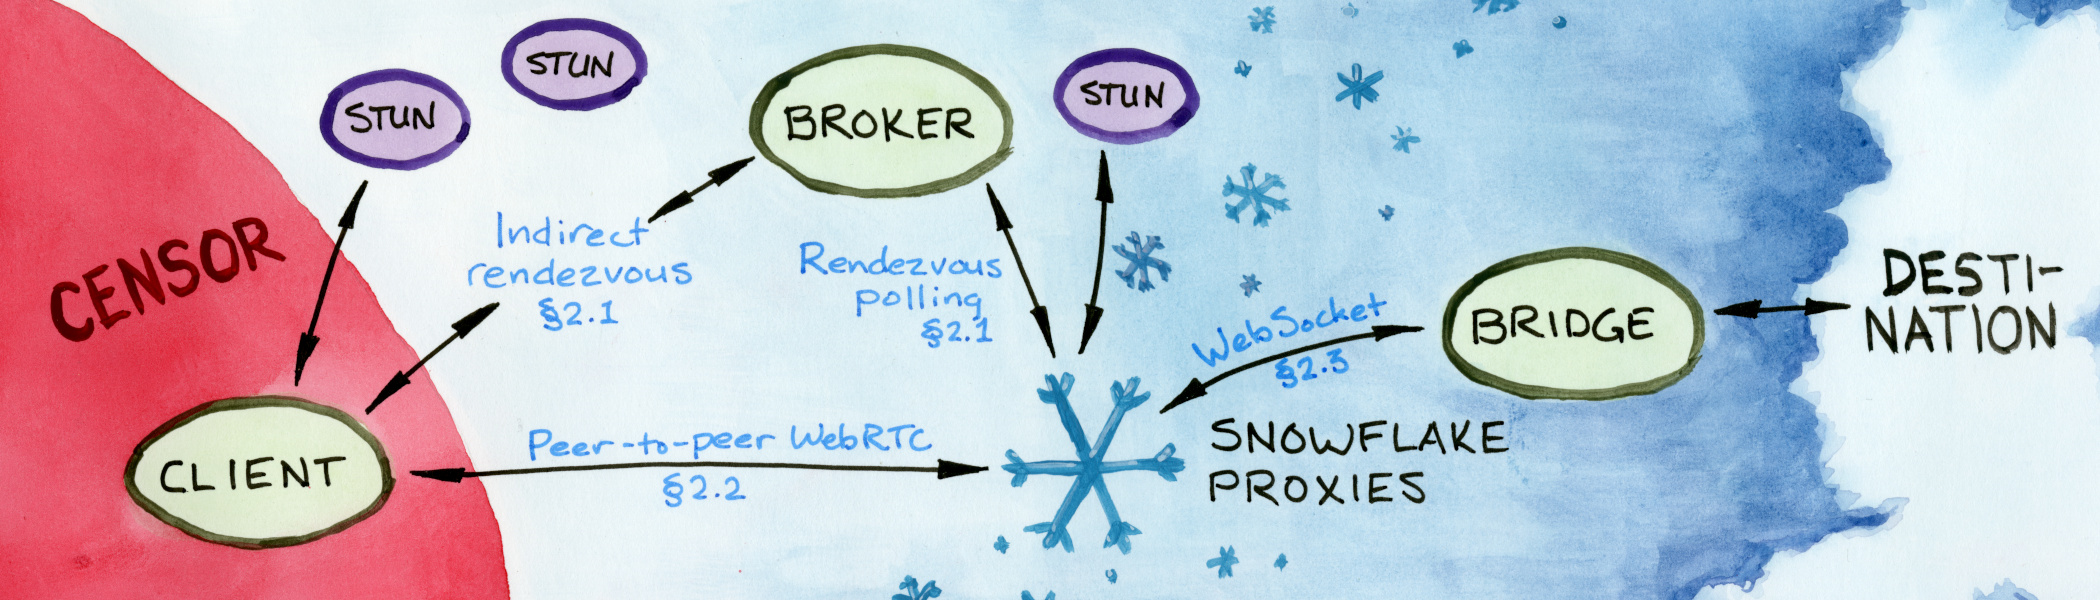
\includegraphics{figures/architecture/architecture.jpg}
\caption{
Architecture of Snowflake.
The client contacts the broker through a special rendezvous channel with high blocking resistance.
The broker matches the client with one of the proxies that are currently polling.
The client and proxy connect to one another using WebRTC.
The proxy connects to the bridge,
then begins copying traffic in both directions.
If~the proxy disappears,
the client does another rendezvous
and resumes its session with a new proxy.
}
\label{fig:architecture}
\end{figure*}

A~Snowflake proxy connection proceeds in three phases.
First, there is rendezvous, in which a client
indicates its need for circumvention service
and is matched with a temporary proxy.
Rendezvous is facilitated by a central server called the broker.
Then, there is connection establishment,
where the client and its proxy connect to each other
with WebRTC, using information exchanged during rendezvous.
Finally, there is data transfer,
where the proxy transports data
between the client and the bridge.
The bridge is responsible for directing the client's traffic
to its eventual destination
(in~our case, by feeding it into the Tor network).
\autoref{fig:architecture} illustrates the process.

These phases repeat as needed, as temporary proxies come and~go.
Proxy failure is not an abnormal condition---it~happens whenever
a proxy is running in a browser that is closed, for example.
A~client builds a circumvention session over
a sequence of proxies, switching to a new one
whenever the current one stops working.
State variables stored at the client and the bridge
let the session can pick up where it left off.
The change of proxies is invisible to the applications using Snowflake
(except for a brief delay while rendezvous happens):
the Snowflake client presents an abstraction of a single, uninterrupted connection.

It~does not avail a censor to block the broker or bridge,
because Snowflake clients never contact either one directly.
Clients reach the broker over an indirect rendezvous channel.
Access to the bridge is always mediated by a temporary proxy.

\subsection{Rendezvous}
\label{sec:rendezvous}

A~session begins with a client sending a rendezvous message to the broker.
There is an ambient population of proxies
constantly polling the broker to check for clients in need of service.
The broker matches the client with an available proxy,
taking into consideration factors like NAT compatibility.
% NAT type is currently the only constraint:
% matchSnowflake https://gitlab.torproject.org/tpo/anti-censorship/pluggable-transports/snowflake/-/blob/9edaee65470a1483bbdbe984e5e15a885f1e95d2/broker/ipc.go#L236
% But protocol versions may become a consideration in the future:
% "Analysis of speed deficiency of Snowflake in China, 2023 Q1" https://bugs.torproject.org/tpo/anti-censorship/pluggable-transports/snowflake/40251#note_2903271

The client's rendezvous message
% ClientPollRequest https://gitlab.torproject.org/tpo/anti-censorship/pluggable-transports/snowflake/-/blob/9edaee65470a1483bbdbe984e5e15a885f1e95d2/common/messages/client.go#L64
is a bundle of data that the broker will need to match the client with a proxy,
and the proxy will need to connect to the client.
The primary element is a
Session Description Protocol (SDP) \firstterm{offer}~\cite{rfc8839},
which contains the information necessary for a WebRTC connection,
including the client's external IP addresses
and cryptographic data to secure a later key exchange.
% Specifically, a certificate fingerprint: https://www.rfc-editor.org/rfc/rfc8122.html#section-5
The broker forwards the client's SDP offer to the proxy,
and the proxy sends back an SDP \firstterm{answer}
with its share of connection details.
The broker forwards the proxy's SDP answer to the client.
The client and proxy then connect to each other directly.
In WebRTC terms, this offer/\allowbreak answer exchange is called
``signaling,'' and here the broker acts as a signaling server.
To~gather the information for an SDP offer or answer,
clients and proxies communicate with third-party servers,
called STUN servers,
before contacting the broker.
We~will say more about how this information is used in \autoref{sec:connection}.
Communication with STUN servers is a normal and expected part of WebRTC,
though there are fingerprinting considerations
that we discuss in \autoref{sec:fingerprinting}.

Interaction with the broker uses a ``long-polling'' model.
An~example is shown in \autoref{fig:rendezvous}.
Proxies poll the broker periodically,
making an HTTPS request to a designated URL path.
The broker does not respond immediately to a proxy poll,
but instead holds the connection idle for a few seconds
to await the possible arrival of a client rendezvous message.
If~none arrives, the broker sends a response saying ``no clients''
and the proxy goes to sleep until its next poll.
When a client does arrive,
the broker sends the SDP offer in response
to the proxy's poll request.
The proxy sends its SDP answer to the broker
in a separate HTTPS request.
The broker responds to the client's pending request
with the proxy's SDP answer,
at~the same time sending an acknowledgement to the proxy.
At~this point rendezvous is finished,
and the client and the proxy may connect to one another.

\begin{figure}
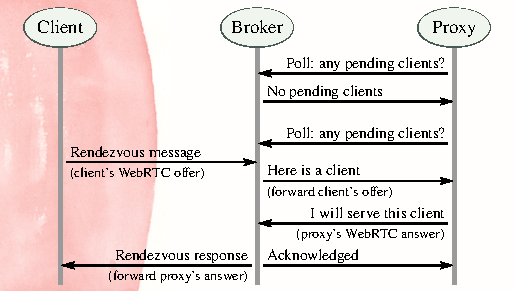
\includegraphics{figures/rendezvous/rendezvous}
\caption{
The long-polling communication model of Snowflake rendezvous.
Proxies poll periodically to check for new clients.
When the broker makes a match,
the proxy gets the client's SDP offer,
then immediately re-connects to send back its SDP answer.
It~all happens during one round trip from the client's perspective.
}
\label{fig:rendezvous}
\end{figure}

The client must use an indirect,
blocking-resistant channel
when communicating with the broker.
What is needed, essentially,
is a miniature circumvention system
to bootstrap the full system.
What makes rendezvous
different from general circumvention
are its different (generally more lenient) requirements,
which permit a larger solution space.
Because rendezvous is only a small fraction
of total communication volume,
and it happens relatively infrequently,
it~may use techniques that would be
too slow, expensive, or complicated
for real-time or bulk data transfer.
Rendezvous is separable and modular:
more than one method can be used,
and the methods do not necessarily need to bear any relation
to the circumvention techniques of the main system.
While the assumption of WebRTC permeates Snowflake's design,
its rendezvous modules are independent.
We~currently support two rendezvous methods in Snowflake:

\begin{description}
\item[Domain fronting]
In~this method, the client does an HTTPS exchange with the broker
through an intermediary web service such as a content delivery network (CDN),
setting the externally visible hostname
(the TLS Server Name Indication, or SNI)
to a ``front domain'' different from the broker's.
The CDN routes the HTTPS request to the broker not according to the TLS SNI
but rather the HTTP Host header, which, under TLS encryption,
reflects the broker's true hostname~\cite{Fifield2015a}.
A~censor cannot easily block domain-fronted rendezvous
without also blocking unrelated connections to the front domain,
which should be selected to have high value to the censor.
(But see \autoref{sec:fingerprinting} for features other than
the hostname that a censor might try to use.)
The well-known drawback of domain fronting
is the high cost of CDN bandwidth.
Because we use it only for rendezvous,
the cost is much less than if we were to use it
for all data transfer.

% "AMP cache rendezvous" https://gitlab.torproject.org/tpo/anti-censorship/pluggable-transports/snowflake/-/merge_requests/50
\item[AMP cache]
AMP is a framework for web pages written in a restricted dialect of HTML.
Part of the framework is a free-to-use
cache server~\cite{amp-cache}.
The cache fetches AMP-conformant web pages on demand,
which means that it is, effectively, a~restricted sort of HTTP proxy.
We~have a module that encodes rendezvous messages to AMP specifications,
allowing them to be exchanged with the broker via the AMP cache.
Rendezvous through the AMP cache is not easily blocked
without blocking the cache server as a whole.
This rendezvous method still technically requires domain fronting,
because the AMP cache protocol would otherwise expose the
broker's hostname in the TLS SNI,
but it increases the number of usable intermediaries and front domains.
\end{description}

Anything that can be persuaded to convey a message
of about 1500 bytes indirectly to the broker,
and return a response of about the same size,
can work as a rendezvous module.
% "Broker: investigate non-domain-fronting secure client / proxy registrations" https://bugs.torproject.org/tpo/anti-censorship/pluggable-transports/snowflake/25594
For example, encrypted DNS
% "DNS-based rendezvous for Snowflake" https://bugs.torproject.org/tpo/anti-censorship/pluggable-transports/snowflake/25874
or a chat bot
% "Example: there is a chat bot (say, Telegram), that acts as a broker." https://bugs.torproject.org/tpo/anti-censorship/pluggable-transports/snowflake/25594#note_2823395
would serve.
Though some systems (flash proxy was one)
may need only a single, outgoing rendezvous message,
Snowflake needs a two-way exchange,
to support the SDP offer and answer.
% Flash proxy email rendezvous would not work for Snowflake, because unidirectional.
% https://gitweb.torproject.org/flashproxy.git/tree/flashproxy-reg-email
% https://gitweb.torproject.org/flashproxy.git/tree/facilitator/fp-registrar-email

Rendezvous is not unique to Snowflake.
Other examples of rendezvous in circumvention include
the DEFIANCE Rendezvous Protocol~\cite[\S 3]{Lincoln2012a},
the facilitator interaction in flash proxy~\cite[\S 3]{Fifield2012a},
and the registration proxy in Conjure~\cite[\S 4.1]{Frolov2019b}.
A~key property of Snowflake and the mentioned systems
is that they do not rely on preshared secret information.
The client needs only to acquire the necessary software;
whatever additional information is required to establish a circumvention session
is exchanged dynamically, at runtime.
This stands in contrast to another class of systems in which,
prior to making a connection,
a~client must acquire some secret,
such as an IP address or password,
through an out-of-band channel
presumed to be unavailable to the censor---and
the system's blocking resistance depends on
keeping that information hidden from the censor.
A~corollary of the no-secret-information property
is that an adversary---the censor---is
at no special disadvantage in attacking the system.
The censor may download the client software,
run it, study its network connections---and
the system must maintain its blocking resistance despite this.
The disadvantage of a separate rendezvous step
is that it is one more thing to get right.
Not only the main circumvention channel
but also the rendezvous must resist blocking:
the system is only as strong as the weaker of the~two.

\subsection{Peer-to-peer connection establishment}
\label{sec:connection}

Now the client and the proxy connect to each other directly.
Even in the absence of censorship,
making a direct connection between two Internet peers is not always easy,
because of NAT (network address translation) and firewalls.
Snowflake clients and proxies alike run in diverse networks
with varying NATs and ingress policies.
Fortunately for us,
WebRTC is designed with this use case in mind,
and has built-in support for traversing NAT, in~the form of
ICE (Interactive Connectivity Establishment)~\cite{rfc8445},
a procedure for testing candidate pairs of peer network addresses
to find one that works.
ICE~makes use of third-party
STUN (Session Traversal Utilities for NAT)~\cite{rfc8489}
servers that, among other things,
enable a host to learn its external IP addresses.
The first part of ICE took place at the beginning of rendezvous,
when the client and proxy contacted STUN servers to gather
external address candidates and included them in their respective
SDP offer and answer.

There is no guarantee that two hosts will be able to make
a connection using the facilities of STUN alone.
Some address mapping and
filtering setups are simply incompatible.
In~such a case,
ICE would normally fall back to using
TURN (Traversal Using Relays around NAT)~\cite{rfc8656},
a~kind of UDP proxy.
Such a fallback would be problematic for Snowflake,
because the TURN relays themselves
would become a target of blocking by the censor.
% "Configure TURN servers for the proxy and/or client" https://bugs.torproject.org/tpo/anti-censorship/pluggable-transports/snowflake/25596
But Snowflake has an advantage most WebRTC applications do not.
Most WebRTC applications want to connect \emph{a particular} pair of peers,
whereas we are satisfied when a client can connect to \emph{any} proxy.
Snowflake clients and proxies self-measure their NAT type
and report it to the broker,
which takes NAT compatibility into account
and avoids cases that would require a fallback to TURN.

% "Investigate Snowflake proxy failures" https://bugs.torproject.org/tpo/anti-censorship/pluggable-transports/snowflake/33666#note_2595319
% "Okay here's a summary of what I've found: ..."

We condense the possible combinations of NAT and firewall features
that impact
a Snowflake client or proxy's
ability to make a peer-to-peer connection
into the following well-known variations:

% https://datatracker.ietf.org/doc/html/rfc3489#section-5
\begin{description}
\item[Full cone]
The same internal IP--port pair always maps to the same external port.
Any remote host may send a packet to an internal IP address and port by sending a packet to the
mapped external port.
\item[Restricted cone]
Like full cone,
but incoming packets
are allowed only if
there has recently been an outgoing packet
to the same remote IP address.
\item[Port-restricted cone]
Like restricted cone,
but incoming packets are allowed only if
there has recently been an outgoing packet
to the same remote IP--port pair.
\item[Symmetric]
The external port depends on both
the internal IP--port pair and the remote IP--port pair.
Incoming packets are allowed only if
there has recently been an outgoing
packet to the same remote address.
\end{description}

\begin{table}
\definecolor{Ycolor}{Gray}{14}
\definecolor{ncolor}{Gray}{13}
\newcommand{\Y}{\cellcolor{Ycolor}\ding{51}}
\newcommand{\n}{\cellcolor{ncolor}--}
\newcommand{\rotlabel}[1]{\rotatebox{30}{#1}}
% \vphantom is to make the labels take up vertical space;
% \rlap is so they don't expand the horizontal size of table columns.
\newcommand{\rot}[1]{\vphantom{\rotlabel{#1}}\rotlabel{\rlap{#1}}}
\centering
% Make normal cells taller by default.
\renewcommand{\arraystretch}{1.25}
% Tighten line spacing in \makecell cells.
\renewcommand\cellset{\renewcommand\arraystretch{0.8}\setlength\extrarowheight{0pt}}
\begin{tabular}{@{}rcccccl@{\hspace{0.5ex}}l@{}}
& % empty
\rot{No NAT} &
\rot{Full cone} &
\rot{Restricted cone} &
\rot{Port-restricted cone} &
\rot{Symmetric} &
&
\\
No NAT               & \Y & \Y & \Y & \Y & \Y & \multirow{3}{*}{\kern-\tabcolsep\kern0.5ex\footnotesize\(\left.\kern-\nulldelimiterspace\rule[-19pt]{0pt}{38pt}\right\}\)} & \multirow{3}{*}{\footnotesize\makecell[l]{unrestricted\\proxy}} \\
Full cone            & \Y & \Y & \Y & \Y & \Y & \\
Restricted cone      & \Y & \Y & \Y & \Y & \Y & \\
Port-restricted cone & \Y & \Y & \Y & \Y & \n & \multirow{2}{*}{\kern-\tabcolsep\kern0.5ex\footnotesize\(\left.\kern-\nulldelimiterspace\rule[-12pt]{0pt}{24pt}\right\}\)} & \multirow{2}{*}{\footnotesize\makecell[l]{restricted\\proxy}} \\
Symmetric            & \Y & \Y & \Y & \n & \n & \\[\dimexpr 0.5ex - \dimexpr 0.5\dimexpr\arraystretch\normalbaselineskip]
% \hfill hack to make \upbracefill work with colortbl:
% https://tex.stackexchange.com/questions/202138/upbracefill-filling-entire-tabular-cell-and-package-colortbl#comment474604_202143
                     & \multicolumn{4}{@{~}c@{~}}{\footnotesize\def\hfill{\hskip 0pt plus 1filll}\upbracefill} & \clap{\footnotesize\def\hfill{\hskip 0pt plus 1filll}\upbracefill} & \\
                     & \multicolumn{4}{c}{\footnotesize\makecell{unrestricted\\client}} & \clap{\footnotesize\makecell{restricted\\client}} \\
\end{tabular}
\caption{
Pairwise compatibility of NAT variants,
using the facilities of STUN alone
(no fallback to TURN).
The incompatible cases are when one peer's NAT is symmetric
and the other's is symmetric or port-restricted cone.
Note the asymmetry in what NAT variants are ``restricted''
in client and proxy.
}
\label{tab:nat-matching}
\end{table}

\autoref{tab:nat-matching}
shows the pairwise compatibility of NAT variations.
As~the incompatible cases always involve a symmetric NAT,
we further simplify matching by categorizing the variations into the two types
\firstterm{unrestricted} (works with most other NATs) and
\firstterm{restricted} (works only with more permissive NATs).
Unrestricted proxies may be matched with any client;
restricted proxies may be matched only with unrestricted clients.
The broker prefers to match unrestricted clients with restricted proxies,
% https://gitlab.torproject.org/tpo/anti-censorship/pluggable-transports/snowflake/-/blob/9edaee65470a1483bbdbe984e5e15a885f1e95d2/broker/ipc.go#L236
in~order to conserve unrestricted proxies
for the clients that need them.
Symmetric NAT is always considered restricted,
but port-restricted cone NAT differs
depending on the peer:
for proxies it is restricted, but
for clients it is unrestricted.
The asymmetric categorization is an approximation
to help conserve unrestricted proxies
for clients with symmetric NATs.
Though it creates the potential for an incompatible match,
we believe this to be uncommon in practice.
In~case of a connection failure,
clients re-rendezvous and try again.

To self-assess their NAT type,
clients use the NAT behavior discovery feature of STUN~\cite{rfc5780}.
% "Use STUN to determine NAT behaviour of peers" https://bugs.torproject.org/tpo/anti-censorship/pluggable-transports/snowflake/34129
% "Add utility to help user discover their NAT type" https://github.com/pion/stun/issues/8
Proxies cannot use the same technique,
because the necessary STUN features are not exposed
to JavaScript.
% "Have a remote probe service to test snowflake proxy NAT compatability" https://bugs.torproject.org/tpo/anti-censorship/pluggable-transports/snowflake/40013
Instead,
we adapt a technique from MassBrowser~\cite[\S \mbox{V-A}]{Nasr2020a}:
we~run a centralized, always-on WebRTC testing peer
behind a simulated symmetric NAT.
Proxies try connecting to this peer:
if~the connection succeeds, the proxy's type is unrestricted;
otherwise it is restricted.

While the proxy is connecting to its client,
% "While": https://gitlab.torproject.org/tpo/anti-censorship/pluggable-transports/snowflake/40228
it also connects to the bridge.
This connection
uses WebSocket~\cite{rfc6455}, which
offers a TCP-like, client--server connection
layered on HTTPS.
The choice of protocol for the proxy--bridge link is arbitrary,
and could be changed
without affecting the rest of the system.
It does not need to be resist blocking,
it~just needs to be available to JavaScript code in web browsers.
WebRTC, for example, would work for this link too.

\subsection{Data transfer}
\label{sec:data-transfer}

No~complicated processing takes place at the proxy.
The main value of a Snowflake proxy is its IP address:
it~gives the client a peer to connect to that is not on the censor's address blocklist.
Having provided that,
the proxy assumes a role of pure data transfer.

Snowflake uses a stack of nested protocol layers.
We~will walk though the layers and describe the purpose of each.

\bigskip

\noindent
\begin{tabular}{@{}l@{\,}l@{}l@{\,}l}
UDP & \rdelim\}{3}{*} & \multirow{3}{5em}{WebRTC data channel} & \rdelim\}{3}{*}[\,ephemeral, per proxy]\\
DTLS \\
SCTP \\
KCP & \rdelim\}{2}{*} & \multirow{2}{*}{Turbo Tunnel} & \rdelim\}{3}{*}[\,persistent, per session] \\
smux \\
\multicolumn{3}{@{}l}{Tor protocol} \\
\multicolumn{4}{@{}l}{application streams} \\
\end{tabular}

\bigskip

\noindent
This is the stack for the client--proxy link,
which is the place where WebRTC is used, and which is
exposed to observation by the censor (\autoref{fig:architecture}).
The stack for the proxy--bridge link is the same,
but with WebSocket in place of the
WebRTC data channel at the top.
The layers marked ``ephemeral'' are skimmed off
and replaced as proxies come and~go.
The layers marked ``persistent'' are instantiated once
in each circumvention session,
hold long-term state,
and are end-to-end between client and bridge.

The connection between a client and its proxy is
a WebRTC data channel~\cite{rfc8831},
which provides a way to send arbitrary binary messages between peers.
A~data channel is its own stack of three protocols:
UDP for network transport,
DTLS (Datagram TLS)
for confidentiality and integrity, and
SCTP (Stream Control Transmission Protocol)
for delimiting message boundaries
and other features like congestion control.
Working UDP port numbers will have been discovered
using ICE in the previous phase.
The peers authenticate one another
at the DTLS layer using certificate fingerprints
that were exchanged during rendezvous~\cite[\S 5.1]{rfc8842}.

Data channels are well-suited to Snowflake's needs.
(The specification even lists circumvention as a use case~\cite[\S 3.2]{rfc8831}.)
But data channels are not the only option:
WebRTC also offers \firstterm{media streams}
for unreliable transport of real-time audio and video.
Which of these is used may be a fingerprinting vector.
We~will take up this topic in \autoref{sec:fingerprinting}.

If~clients only ever used one proxy,
a~WebRTC data channel alone would be sufficient.
But a Snowflake proxy might
disappear at any moment,
and when that happens, its data channel goes with~it.
If~the client was in the middle of a long download,
for example, it should be possible to resume the download
without interruption after rendezvousing with a new proxy.
For this we need a shared notion of session state that exists
at the client and the bridge, not tied to any temporary proxy.
A~lack of session continuity across proxy failures
had been an unsolved problem in flash proxy~\cite[\S 5.2]{Fifield2012a}.

We~adopt the
Turbo Tunnel design pattern~\cite{Fifield2020a}
and insert a userspace
session and reliability protocol
between the ephemeral proxy data channels
and the client's own application streams.
% "[anti-censorship-team] Turbo Tunnel in Snowflake" https://lists.torproject.org/pipermail/anti-censorship-team/2020-February/000059.html
This part of the protocol stack
outlives any single proxy; it~belongs to
the client and the bridge.
Its primary function is to attach sequence numbers and acknowledgements
to packets of data,
so~that both ends know what parts of the data stream
need to be retransmitted after a temporary loss of proxy connectivity.
The client tags its traffic
with a random session identifier string that remains
consistent throughout a session,
which the bridge uses to index a map of session variables.
For the inner session layer we use a combination of
KCP~\cite{kcp} and
smux~\cite{smux}.
KCP provides reliability,
and smux detects the end of idle sessions and terminates them.
KCP and smux have shown their worth in other deployments,
and are easy to program,
but there is nothing about them on which we depend essentially.
Any other transport protocol that provides the necessary features
and can be implemented in userspace would~do,
such as QUIC, TCP, or (another layer~of) SCTP.
We~prototyped successfully with QUIC before deciding on KCP/\allowbreak smux.

% Not going to get into how we currently use reliable, ordered (TCP-like) data
% channels, but plan to switch to unreliable, unordered (UDP-like) data
% channels, a better fit for the underlying datagram-oriented Turbo Tunnel
% layer.
%
% "turn off reliable mode for WebRTC DataChannel" https://gitlab.torproject.org/tpo/anti-censorship/pluggable-transports/snowflake/-/merge_requests/109
% "Snowflake is currently using network resource in a so suboptimal way..." https://bugs.torproject.org/tpo/anti-censorship/pluggable-transports/snowflake/40251#note_2891751

Snowflake can be seen as an instance of the
``untrusted messengers'' model of Feamster et~al.~\cite[\S 3]{Feamster2003a}:
our \firstterm{proxies} and \firstterm{bridge} correspond to their
\firstterm{messengers} and \firstterm{portal}.
Proxies are tasked with delivering the client's data to the bridge,
but are not permitted to tamper with or inspect~it,
which necessitates an inner,
end-to-end secure protocol between the client and the bridge.
In~our deployment, this is Tor protocol.
After removing the WebSocket and Turbo Tunnel layers,
the Snowflake bridge feeds the client's Tor streams
into a Tor bridge running on the same host.
The use of Tor is an implementation choice, not a requirement---many
other protocols would work in its place.
Tor has the nice quality that
not even the bridge
sees the plaintext of client streams.
But Tor also has certain drawbacks,
which we will comment on in
\autoref{sec:future}.

\section{Protocol fingerprinting}
\label{sec:fingerprinting}

% https://gitlab.torproject.org/tpo/anti-censorship/pluggable-transports/snowflake/-/wikis/Fingerprinting

Snowflake leans heavily into the ``address blocking'' side of circumvention,
but the ``content blocking'' part matters too.
The goal, as~always, is to make circumvention traffic
difficult to distinguish from other traffic the censor cares not to block.
Snowflake is inherently tied to WebRTC,
and can only be effective against a censor
that is not willing to block WebRTC protocols wholesale.
But even within that scope,
there are many variations in \emph{how}
WebRTC is implemented and used,
which, if~not carefully considered, might enable a censor
to selectively block only Snowflake,
while leaving other uses of WebRTC undisturbed.
Unfortunately for the circumvention developer,
the richness of WebRTC protocols
affords a large attack surface for fingerprinting.
Not only that, WebRTC leaves the details of
signaling---in~which peers exchange information
needed to set up a connection,
corresponding to Snowflake rendezvous---unspecified~\cite[\S 3]{rfc8825},
leaving every application to invent its own mechanism.
% "The choice of protocols for client-server and inter-server signaling, and the definition of the translation between them, are outside the scope of the WebRTC protocol suite described in this document."
% https://www.rfc-editor.org/rfc/rfc8829.html#section-3.1: "JSEP does not specify a particular signaling model or state machine, other than the generic need to exchange session descriptions in the fashion described by [RFC3264] (offer/answer)..."

As~WebRTC is designed for the web,
most implementations of WebRTC are embedded in web browsers,
and are not easily removed from that context.
Snowflake originally used a WebRTC library extracted from Chromium,
but that eventually proved unworkable for cross-platform deployment.
Since~2019, Snowflake has used Pion~\cite{pion-webrtc},
% "Evaluate pion WebRTC" https://bugs.torproject.org/tpo/anti-censorship/pluggable-transports/snowflake/28942
an independent implementation of WebRTC
not tied to any browser.
This is both good and bad.
The good is greater agility and less development friction,
and a working relationship with upstream developers
that enables us to get fingerprinting-related changes made;
we~would not be where we are today without~it.
The bad is that the WebRTC fingerprint of Pion
does not automatically match that of the mainly browser-originated
WebRTC that Snowflake aims to blend in with.

The following is a list of fingerprinting concerns
that bear on Snowflake, together with
how we have tried to address them.
The existence of a fingerprinting vulnerability
does not automatically invalidate a circumvention system:
censorship and circumvention are a dialog,
and even among demonstrable vulnerabilities,
some are more and some are less practical for a censor to take advantage~of.
The important thing is to have a solid foundation;
minor flaws may be patched up as necessary.

\begin{description}
\item[Selection of STUN servers]
It~is not unusual for a WebRTC application to use STUN,
but the choice of what STUN servers to use is up to the application.
Running dedicated STUN servers just for Snowflake would not work,
because a censor would experience no collateral harm in
simply blocking them by IP address.
Our deployment uses a pool of public STUN servers
that are used in applications other than circumvention,
filtered for those that support the NAT behavior discovery feature
described in \autoref{sec:connection}.
The client chooses a random subset of servers from the pool
when it makes a connection;
this is because not every STUN server is accessible
under every censor.
% I went to check stun.l.google.com for blocking in China,
% but OONI Probe does not measure that server as of v3.17.1:
% https://github.com/ooni/probe/issues/2417#issuecomment-1468478811

\item[Format of STUN messages]
STUN is most often deployed over plaintext UDP,
which leaves its messages open to inspection
and potential fingerprinting.
STUN messages consist of a fixed header
followed by a variable-length list of ordered
attributes~\cite[\S 5]{rfc8489}.
What attributes appear,
and their order,
depends on the STUN implementation
and how the application uses it.

We have not done anything in particular
to disguise STUN messages.
Though plaintext UDP is the most common,
STUN specifies other transports,
including encrypted ones like DTLS.
These may be options for Snowflake in the future---of~course,
only if they are common enough that their use
does not stick out on its own.
% "Investigate if STUN over TCP/TLS is beneficial to us" https://bugs.torproject.org/tpo/anti-censorship/pluggable-transports/snowflake/40240

\item[Rendezvous]
Because the rendezvous methods of
\autoref{sec:rendezvous}
are modular,
each one needs a separate justification
as to why it should be difficult to block.
Besides that, they must be implemented in a way
that does not expose accidental distinguishers.
For example, the domain fronting and AMP cache rendezvous methods
use HTTPS, which is TLS,
which means TLS fingerprinting is a concern~\cite[\S 5.1]{Fifield2015a}.
Snowflake, like many circumvention systems,
uses the uTLS package~\cite[\S VII]{Frolov2019a}
to get a client TLS fingerprint that is randomized or that imitates common browsers.
See \autoref{sec:block-ir} for an account of when
domain fronting rendezvous was briefly blocked in Iran,
because we were slow in activating uTLS.

Though each rendezvous method may be difficult to block in itself,
a~censor might combine a low-confidence detection of rendezvous
with features from other phases of the Snowflake data exchange
to strengthen its guess.

\item[DTLS]
The outermost layer of a WebRTC data connection,
the protocol directly exposed to a censor,
is DTLS (Datagram TLS) over UDP.
DTLS is an adaptation of TLS~\cite[\S 1]{rfc9147} to the datagram setting,
and therefore inherits the fingerprinting concerns of TLS~\cite{Frolov2019a}.
TLS/DTLS fingerprinting may involve, for example,
inspecting ClientHello messages to see what
ciphersuites and extensions are used,
and their order. It~may be that a certain combination
is specific to a particular implementation of a circumvention system,
and may therefore be blocked at low cost.

Due to practical considerations,
Snowflake's defenses to DTLS fingerprinting are not very robust,
and are reactive rather than proactive.
In~the realm of TLS one may use uTLS,
but there is as yet no equivalent of uTLS for DTLS.
The present way of altering DTLS fingerprints in Snowflake
is to submit a pull request upstream to Pion
whenever a fingerprint feature used for blocking is identified.
\autoref{sec:block-ru} documents how this has happened twice already,
in response to blocking in Russia.

% For reference, fingerprinting changes upstreamed to Pion:
% * IP addresses as SNI values
%   https://bugs.torproject.org/tpo/anti-censorship/pluggable-transports/snowflake/40014#note_2764715
%   https://github.com/pion/dtls/issues/406
%   https://github.com/pion/dtls/pull/407
% * supported_groups in Server Hello
%   https://bugs.torproject.org/tpo/anti-censorship/pluggable-transports/snowflake/40014#note_2765074
%   https://github.com/pion/dtls/issues/409
%   https://github.com/pion/dtls/pull/410
% * Server sending Hello Verify Request
%   https://bugs.torproject.org/tpo/anti-censorship/pluggable-transports/snowflake/40014#note_2764715
%   https://gitlab.torproject.org/tpo/applications/tor-browser-build/-/merge_requests/637
%   https://bugs.torproject.org/tpo/anti-censorship/pluggable-transports/snowflake/40249
%   https://github.com/pion/dtls/pull/513
%   https://github.com/pion/webrtc/pull/2407
%
% Not fingerprinting but also upstreamed:
% * NAT behavior detection
%   https://github.com/pion/stun/issues/8
%   https://github.com/pion/stun/pull/33

\item[Data channel or media stream]
Besides data channels, WebRTC offers \firstterm{media streams},
in line with its intended purpose of enabling real-time
audio and video communication.
Though both are encrypted,
data channels and media streams are externally distinguishable
because they use different containers.
Data channels use DTLS,
and media streams use DTLS-SRTP;
that is, the Secure Real-Time Transport Protocol
with a DTLS key exchange~\cite[\S 4.3]{rfc8827}.

Data channels are a closer match to Snowflake's communication model:
media streams are meant to contain encoded audio and video,
not arbitrary binary data.
But the use of DTLS rather than DTLS-SRTP could become
a significant feature if most other WebRTC applications use media streams.
Although it would be less convenient,
it would be possible to adapt the WebRTC link between
the client and its proxy
to use a media stream rather than a data channel,
either by modulating binary data into a well-formed encoded
audio or video signal in the manner~of, say,
Stegozoa~\cite[\S 3.3]{Figueira2022a},
or by directly replacing the ciphertext of SRTP packets,
as in Protozoa~\cite[\S 4.4]{Barradas2020a}.
% See idea about WebRTC Encoded Transform: https://lists.torproject.org/pipermail/anti-censorship-team/2023-February/000284.html

\end{description}

Protocol fingerprinting
is~where most research on detecting Snowflake has focused.
Fifield and Gil Epner~\cite{arxiv.1605.08805}
studied the network traffic of WebRTC applications,
with the goal of finding fingerprinting pitfalls
that might affect Snowflake, at~that time in early development.
Frolov et~al.~\cite[\S \mbox{V-C}]{Frolov2019a}
observed that the unprotected TLS fingerprint
of domain fronting rendezvous was distinctive,
and introduced the uTLS package that Snowflake
now uses to protect it.
MacMillan et~al.~\cite{arxiv.2008.03254}
focused on the DTLS handshake,
comparing Snowflake to three other WebRTC applications.
They correctly anticipated features
of the Pion DTLS handshake
that would later actually be used
to block Snowflake in Russia;
see more details in \autoref{sec:block-ru}.

Chen et~al.~\cite{Chen2023a}
combined features
of rendezvous and DTLS
in order to reduce false positives.
Their classifier begins
by looking for DNS queries for
STUN servers and front domains typically used by Snowflake clients.
They then apply a machine learning classifier
to features of a subsequent DTLS handshake.
The authors acknowledge that DTLS fingerprinting
is fragile, as~the DTLS fingerprint is, in~principle,
controllable by the application.
The DNS prefilter may perhaps be mitigated
by alternative rendezvous methods (\autoref{sec:rendezvous}),
or~by smarter selection of STUN servers.
Xie et~al.~\cite{Xie2023a} trained a decision tree on
packet size, direction, latency, and bandwidth features, with the aim of
distinguishing Snowflake's domain fronting rendezvous
from other forms of HTTPS.
A~challenge in classifying rendezvous flows
is that they do not consist of many packets,
limiting the number of features a classifier has to work with.
Their lowest reported false positive rate of 0.25\%~is,
in~our opinion, unworkably high,
given the low base rate of Snowflake rendezvous connections.

Wails et~al.~\cite{Wails2024a}
criticize past research on classification of circumvention systems,
saying that accuracy claims do not hold up
with the low base rates of circumvention traffic in practice.
% IV-D: "Despite the prima facie acceptable performance of these
% classifiers ... we argue that these results *do not* accurately
% reflect a censor's ability to detect obfs4 under realistic conditions."
They develop classifiers based on deep learning
that improve on the state of the art,
applying them to Snowflake rendezvous and data transfer,
but find them still to be prohibitively imprecise with realistic base rates.
% V-C: "While it is the case that deep learning improves performance,
% the false positive rates are still prohibitively high to scale to
% realistic base rates. Fig. 5 plots Prec^λ as a function of the base
% rate λ. For more realistic base rates, such as λ > 1 × 10^6, the
% precision attained by any of the classifiers is near-zero."
They propose to reduce false positives by combining
multiple observations per IP address---classifying hosts,
not flows---and suggest that Snowflake's lack of
fixed proxies mitigates against this enhancement.
% VII: "One way to mitigate the effects of host-based analysis is to
% design circumvention systems to use multiple ephemeral bridges
% over time rather than a few long-term static bridges, similar
% the design of Snowflake.

\begin{figure*}[t]
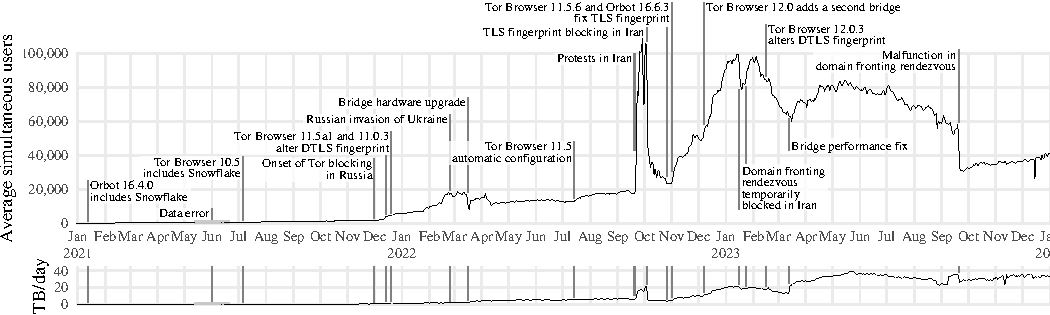
\includegraphics{figures/users/users-global}
\caption{
Estimated average simultaneous Snowflake users and bandwidth by day.
}
\label{fig:client-counts}
\end{figure*}

\section{Experience}
\label{sec:experience}

Snowflake has now been in operation for a few years.
In~lieu of a forward-looking evaluation,
here we take a look back
at the history of our deployment
and reflect on the experience.

\subsection{Client counts and bandwidth}
\label{sec:clients}

% Excerpts from https://gitlab.torproject.org/tpo/network-health/metrics/timeline:
% |2017-01-24|||snowflake|Tor Browser 7.0a1 released, including Snowflake for GNU/Linux only.|[blog post](https://blog.torproject.org/blog/tor-browser-70a1-released)||
% |2017-08-08|||snowflake|Tor Browser 7.5a4 released, including Snowflake for macOS.|[blog post](https://blog.torproject.org/blog/tor-browser-75a4-released) [issue](https://bugs.torproject.org/tpo/applications/tor-browser/22831)||
% |2018-03-26 20:43:42|||snowflake|Release of Tor Browser 8.0a5. Improves snowflake client performance.|[blog post](https://blog.torproject.org/tor-browser-80a5-released) [ticket](https://bugs.torproject.org/tpo/anti-censorship/pluggable-transports/snowflake/21312)||
% |2019-10-01|||snowflake|Release of Tor Browser 9.0a7, the first release that has Snowflake for Windows.|[blog post](https://blog.torproject.org/new-release-tor-browser-90a7) [ticket](https://bugs.torproject.org/tpo/anti-censorship/pluggable-transports/snowflake/25483)||
% |2020-05-22 19:51:29|||snowflake|Release of Tor Browser 9.5a13, the first release with Turbo Tunnel session persistence features for Snowflake. There is a spike in estimated users on 2020-05-21 and 2020-05-22, which appears to be an artifact.|[blog post](https://blog.torproject.org/new-release-tor-browser-95a13) [ticket](https://bugs.torproject.org/tpo/applications/tor-browser/34043) [users graph](https://metrics.torproject.org/userstats-bridge-transport.html?start=2020-03-01&end=2020-08-01&transport=snowflake)||
% |2020-06-02 18:09:48|||snowflake|Release of Tor Browser 10.0a1, the first release with Snowflake for Android.|[blog post](https://blog.torproject.org/new-release-tor-browser-100a1) [ticket](https://bugs.torproject.org/tpo/applications/tor-browser/30318)||
% |2020-06-25|2020-06-25||snowflake|One- or two-day spike in estimated Snowflake users. It resembles the spike that occurred around the time of the Turbo Tunnel release of Tor Browser 9.5a13 on 2020-05-22.|[users graph](https://metrics.torproject.org/userstats-bridge-transport.html?start=2020-03-01&end=2020-08-01&transport=snowflake)|X|
% |2020-08-19|||snowflake|Release of Tor Browser 10.0a5, which added added the ability to do NAT behavior discovery to the Snowflake client.|[blog post](https://blog.torproject.org/new-release-tor-browser-100a5/) [issue](https://bugs.torproject.org/tpo/applications/tor-browser-build/40016)||
% |2020-10-29|||snowflake|Release of Snowflake WebExtension 0.5.0, with a NAT type self-test.|[archive](https://archive.org/details/snowflake-webextension-0.5.0) [issue](https://bugs.torproject.org/tpo/anti-censorship/pluggable-transports/snowflake/40013)||
% |2020-11-17|||snowflake|Release of Snowflake WebExtension 0.5.2, with a fix to the NAT type self-test.|[archive](https://archive.org/details/snowflake-webextension-0.5.2) [merge request](https://gitlab.torproject.org/tpo/anti-censorship/pluggable-transports/snowflake-webext/-/merge_requests/9) [comment](https://bugs.torproject.org/tpo/anti-censorship/pluggable-transports/snowflake/40013#note_2716071)||
% |2021-01-12|||snowflake|Release of Orbot 16.4.0-RC-1-tor-0.4.4.6, first release with Snowflake client support.|[release](https://github.com/guardianproject/orbot/releases/tag/16.4.0-RC-1-tor-0.4.4.6)||
% |2021-02-23|||snowflake|Release of Orbot 16.4.1-BETA-2-tor.0.4.4.6, with experimental Snowflake proxy support.|[release](https://github.com/guardianproject/orbot/releases/tag/16.4.1-BETA-2-tor.0.4.4.6)||
% |2021-07-06 16:56:37|||snowflake|Release of Tor Browser 10.5, first stable release that includes Snowflake.|[blog post](https://blog.torproject.org/new-release-tor-browser-105)||
% |2021-12-01|ongoing|ru||Blocking of Tor directory authorities, relays, default obfs4 bridges, meek-azure, and Snowflake in some ISPs in Russia. There was a temporary cease of blocking for less than a day starting on 2021-12-08.|[NTC thread](https://ntc.party/t/ooni-reports-of-tor-blocking-in-certain-isps-since-2021-12-01/1477) [BBS thread](https://github.com/net4people/bbs/issues/97) [issue](https://bugs.torproject.org/tpo/community/support/40050) [blog post](https://blog.torproject.org/tor-censorship-in-russia/) [OONI report](https://ooni.org/post/2021-russia-blocks-tor/#blocking-of-the-tor-network)||
% |2021-12-14|||snowflake|Release of Tor Browser 11.5a1, with an altered DTLS fingerprint in Snowflake to counteract blocking in Russia.|[blog post](https://blog.torproject.org/new-release-tor-browser-115a1/) [issue](https://bugs.torproject.org/tpo/applications/tor-browser-build/40393) [NTC post](https://ntc.party/t/ooni-reports-of-tor-blocking-in-certain-isps-since-2021-12-01/1477/59)||
% |2021-12-20|||snowflake|Release of Tor Browser 11.0.3, with an altered DTLS fingerprint in Snowflake to counteract blocking in Russia.|[blog post](https://blog.torproject.org/new-release-tor-browser-1103/) [issue](https://bugs.torproject.org/tpo/applications/tor-browser-build/40393) [NTC post](https://ntc.party/t/ooni-reports-of-tor-blocking-in-certain-isps-since-2021-12-01/1477/59)||
% |2022-01-25 17:41:00|||snowflake|Switched the snowflake bridge to a temporary load-balanced staging server. Debugged connection problems until 2022-01-25 18:47:00.|[issue](https://bugs.torproject.org/tpo/tpa/team/40598#note_2772287) [comment](https://bugs.torproject.org/tpo/anti-censorship/pluggable-transports/snowflake/40095#note_2772325) [post](https://forum.torproject.net/t/tor-relays-how-to-reduce-tor-cpu-load-on-a-single-bridge/1483/16) [comment](https://github.com/net4people/bbs/issues/103#issuecomment-1033067920)||
% |2022-03-16 16:51:35|||snowflake|Moved Snowflake traffic to the interim bridge running instances flakey1–flakey8.|[comment](https://bugs.torproject.org/tpo/tpa/team/40664#note_2787624)||
% |2022-05-06 12:14:51|||snowflake|Upgraded the network uplink of the Snowflake bridge from 1 Gbps to 10 Gbps.|[issue](https://bugs.torproject.org/tpo/anti-censorship/pluggable-transports/snowflake/40138)||
% |2022-06-27|||snowflake|Deployed version 0.6.0 of the Snowflake WebExtension. The main feature added in this release was support for more than one bridge. It had a bug that caused it to stop reporting client IP addresses, which are used for metrics purposes by the bridge.|[archive](https://archive.org/details/snowflake-webextension-0.6.0) [merge request](https://gitlab.torproject.org/tpo/anti-censorship/pluggable-transports/snowflake-webext/-/merge_requests/29) [issue](https://bugs.torproject.org/tpo/anti-censorship/pluggable-transports/snowflake-webext/82)||
% |2022-07-14|||bridge|Release of Tor Browser 11.5, with a new feature of automatic censorship circumvention configuration.|[blog post](https://blog.torproject.org/new-release-tor-browser-115/)||
% |2022-09-21|ongoing|ir||Protests and daily Internet shutdowns in Iran.|[OONI report](https://ooni.org/post/2022-iran-blocks-social-media-mahsa-amini-protests/) [BBS thread](https://github.com/net4people/bbs/issues/125)||
% |2022-10-03 12:50:34|||snowflake|Deployment of Snowflake broker to reject proxies that do not support multiple bridges.|[issue](https://bugs.torproject.org/tpo/anti-censorship/pluggable-transports/snowflake/40193) [issue](https://bugs.torproject.org/tpo/anti-censorship/team/95)||
% |2022-10-04 17:15:00|||snowflake|Snowflake rendezvous blocked by TLS fingerprint in Iran.|[issue](https://bugs.torproject.org/tpo/anti-censorship/pluggable-transports/snowflake/40207) [BBS thread](https://github.com/net4people/bbs/issues/131)||
% |2022-10-12|||snowflake|Release of Tor Browser 11.5.4. Adds uTLS TLS camouflage support for Snowflake, making a manual configuration possible to circumvent recent TLS blocking in Iran.|[blog post](https://blog.torproject.org/new-release-tor-browser-1154/) [BBS comment](https://github.com/net4people/bbs/issues/131#issuecomment-1280391051)||
% |2022-10-17 15:52:00||ir|snowflake|Enabled uTLS for Snowflake in Iran in the Circumvention Settings API, using the `hellochrome_auto` fingerprint.|[comment](https://bugs.torproject.org/tpo/anti-censorship/team/96#note_2844378) [merge request](https://gitlab.torproject.org/tpo/anti-censorship/rdsys-admin/-/merge_requests/6)||
% |2022-10-20 15:16:00|||snowflake|Release of Orbot for Android 16.6.3-BETA-2-tor.0.4.7.10. Adds uTLS TLS camouflage support for Snowflake, making it possible to circumvent recent TLS blocking in Iran.|[release](https://github.com/guardianproject/orbot/releases/tag/16.6.3-BETA-2-tor.0.4.7.10) [announcement](https://github.com/net4people/bbs/issues/125#issuecomment-1285897627)||
% |2022-10-27|||snowflake|Release of Tor Browser 11.5.6. Fixes the problem that prevented Snowflake from working in 11.5.5, and enables uTLS TLS camouflage support by default for Snowflake.|[blog post](https://blog.torproject.org/new-release-tor-browser-1156/) [issue](https://bugs.torproject.org/tpo/applications/tor-browser-build/40665)||
% |2022-11-01||ir|snowflake|Orbot begins a gradual release rollout of version 16.6.3-RC-1-tor.0.4.7.10, which has TLS fingerprint changes to make Snowflake work in Iran again.|[release](https://github.com/guardianproject/orbot/releases/tag/16.6.3-RC-1-tor.0.4.7.10)||
% |2022-12-01|||snowflake|Release of Tor Browser 12.0a5, the first release to contain both the snowflake-01 and snowflake-02 bridges.|[issue](https://bugs.torproject.org/tpo/applications/tor-browser-build/40674) [announcement](https://lists.torproject.org/pipermail/tor-announce/2022-December/000256.html) [BBS comment](https://github.com/net4people/bbs/issues/152#issuecomment-1336220171)||
% |2022-12-07|||snowflake|Release of Tor Browser 12.0, the first stable release to contain both the snowflake-01 and snowflake-02 bridges.|[issue](https://bugs.torproject.org/tpo/applications/tor-browser-build/40674) [blog post](https://blog.torproject.org/new-release-tor-browser-120/) [BBS comment](https://github.com/net4people/bbs/issues/152#issuecomment-1342800169) [NTC comment](https://ntc.party/t/second-snowflake-bridge-available-for-testing/3445/2)||
% |2023-01-16|2023-01-24|ir|moat snowflake|The domain name cdn.sstatic.net, which is used by Snowflake and Moat, is blocked in some ISPs in Iran.|[comment](https://bugs.torproject.org/tpo/anti-censorship/team/115#note_2873040)||
% |2023-01-31|2023-02-01|ir|moat snowflake|The domain name cdn.sstatic.net, which is used by Snowflake and Moat, is again blocked in some ISPs in Iran.|[comment](https://bugs.torproject.org/tpo/anti-censorship/team/115#note_2876012)||
% |2023-02-08|2023-02-13|ir|moat snowflake|The domain name cdn.sstatic.net, which is used by Snowflake and Moat, is again blocked in some ISPs in Iran.|[comment](https://bugs.torproject.org/tpo/anti-censorship/team/115#note_2883298) [OONI chart](https://explorer.ooni.org/chart/mat?probe_cc=IR&since=2023-01-23&until=2023-03-01&time_grain=day&axis_x=measurement_start_day&test_name=web_connectivity&domain=cdn.sstatic.net)||
% |2023-02-15|||snowflake|Release of Tor Browser 12.0.3. Has a change to the Snowflake DTLS fingerprint (removes Hello Verify Request) to mitigate reported blocking in Russia.|[blog post](https://blog.torproject.org/new-release-tor-browser-1203/) [comment about Hello Verify Request](https://bugs.torproject.org/tpo/anti-censorship/censorship-analysis/40030#note_2823140) [Snowflake merge request](https://gitlab.torproject.org/tpo/anti-censorship/pluggable-transports/snowflake/-/merge_requests/134) [Tor Browser merge request](https://gitlab.torproject.org/tpo/applications/tor-browser-build/-/merge_requests/637)||
% |2023-02-19|2023-02-19|ir|moat snowflake|The domain name cdn.sstatic.net, which is used by Snowflake and Moat, is again blocked in some ISPs in Iran.|[comment](https://bugs.torproject.org/tpo/anti-censorship/team/115#note_2883298) [OONI chart](https://explorer.ooni.org/chart/mat?probe_cc=IR&since=2023-01-23&until=2023-03-01&time_grain=day&axis_x=measurement_start_day&test_name=web_connectivity&domain=cdn.sstatic.net)||
% |2023-02-22|2023-02-22|ir|moat snowflake|The domain name cdn.sstatic.net, which is used by Snowflake and Moat, is again blocked in some ISPs in Iran.|[comment](https://bugs.torproject.org/tpo/anti-censorship/team/115#note_2883298) [OONI chart](https://explorer.ooni.org/chart/mat?probe_cc=IR&since=2023-01-23&until=2023-03-01&time_grain=day&axis_x=measurement_start_day&test_name=web_connectivity&domain=cdn.sstatic.net)||
% |2023-03-13 19:46:07|||snowflake|Restarted snowflake-02 bridge for a bugfix.|[comment](https://bugs.torproject.org/tpo/anti-censorship/pluggable-transports/snowflake/40262#note_2886032) [issue](https://bugs.torproject.org/tpo/anti-censorship/pluggable-transports/snowflake/40260)||
% |2023-03-13 20:17:54|||snowflake|Restarted snowflake-01 bridge for a bugfix.|[comment](https://bugs.torproject.org/tpo/anti-censorship/pluggable-transports/snowflake/40262#note_2886041) [issue](https://bugs.torproject.org/tpo/anti-censorship/pluggable-transports/snowflake/40260)||
% |2023-03-15|||snowflake|Release of Orbot for Android v17 BETA 2. First release of Orbot to include the snowflake-02 bridge along with the existing snowflake-01. Has a change to the Snowflake DTLS fingerprint (removes Hello Verify Request) to mitigate reported blocking in Russia.|[release](https://github.com/guardianproject/orbot/releases/tag/17.0.0-BETA-2-tor.0.4.7.11) [Orbot commit adding snowflake-02](https://github.com/guardianproject/orbot/commit/c3f6ee18f17770a5904ad19c3cd24b9c8dcb3885) [IPtProxy commit upgrading Snowflake](https://github.com/tladesignz/IPtProxy/commit/5d0654a6a1439c05d3ee52b2b351b5df1ff3f6dc)||

Snowflake became available to end users gradually,
reflecting a long development process.
Development began in late 2015,
% 2015-10-01 initial commit in go-webrtc https://github.com/keroserene/go-webrtc/commit/a044c5aaa6cd8b7c66ca7863e35e1f1931677fc6
% 2015-12-22 initial commit in snowflake https://gitlab.torproject.org/tpo/anti-censorship/pluggable-transports/snowflake/-/commit/41c7613db85f6c1e8d13ea3639fb35d71f6ad942
and deployment in~2017,
but the system only really became usable in~2020.
It~began to attract large numbers of users
(enough to merit a censor's attention)
in~2022, following generalized
network blocking events in Russia and Iran.

Snowflake shipped in the alpha release series of Tor Browser
before graduating to the stable series.
It~was first released for GNU/Linux
in Tor Browser~7.0a1 on \mbox{2017-01-24},
% "First working bundles with Snowflake, for linux only" https://bugs.torproject.org/tpo/anti-censorship/pluggable-transports/snowflake/19001
% "Add snowflake pt to alpha linux builds" https://bugs.torproject.org/tpo/applications/tor-browser/20735
and for macOS
in Tor Browser~7.5a4 on \mbox{2017-08-08}.
% "mac reproducible build" https://bugs.torproject.org/tpo/anti-censorship/pluggable-transports/snowflake/19001
% "[tbb-dev] Please check reproducibility of mac build with Snowflake (e084e83418)" https://lists.torproject.org/pipermail/tbb-dev/2017-July/000579.html
% "Merge Snowflake for mac" https://bugs.torproject.org/tpo/applications/tor-browser/22831
But we hit a roadblock in attempting to prepare releases for other platforms:
the Chromium-derived WebRTC library we had used to that point
presented major difficulties
in Tor Browser's
cross-compiling, reproducible build environment.
What let us resume making progress was a switch to
Pion WebRTC~\cite{pion-webrtc} in~2019.
With it, we~were able to release
Snowflake for Windows
in Tor Browser~9.0a7 on \mbox{2019-10-01},
% "Android reproducible build of Snowflake" https://bugs.torproject.org/tpo/applications/tor-browser/28672
% "Integrate snowflake into mobile Tor Browser alpha" https://bugs.torproject.org/tpo/applications/tor-browser/30318
and for Android in
Tor Browser~10.0a1 on \mbox{2020-06-02}.

While at this point Snowflake was available
on every platform supported by Tor Browser,
it was not yet comfortably usable.
There were two important parts missing:
no NAT type matching (\autoref{sec:connection})
meant that a client could not always connect to its assigned proxy;
and a lack of persistent session state (\autoref{sec:data-transfer})
meant that even if a proxy connection was successful,
the client's session would end once that proxy disappeared.
For these reasons, by early 2020,
the average number of concurrent users
had not risen above~40.
% > library("tidyverse")
% > WANTED_FINGERPRINTS <- c(
%     "7659DA0F96B156C322FBFF3ACCC9B9DC01C27C73" = "snowman",
%     "5481936581E23D2D178105D44DB6915AB06BFB7F" = "snowflake-01",
%     "91DA221A149007D0FD9E5515F5786C3DD07E4BB0" = "snowflake-02"
%   )
% > userstats <- read_csv("figures/users/userstats-bridge-transport-multi.csv") %>%
%     filter(transport == "snowflake" & fingerprint %in% names(WANTED_FINGERPRINTS)) %>%
%     mutate(users = users / (coverage / pmax(num_instances, coverage))) %>%
%     group_by(date, transport) %>% summarize(users = sum(users, na.rm = TRUE), .groups = "drop")
%
% Ignoring two apparently anomalous spikes before 2021.
% One on 2020-05-21 and 2020-05-22 (the day of the Turbo Tunnel release):
% > filter(userstats, "2020-05-19" <= date & date <= "2020-05-24")
% # A tibble: 6 x 3
%   date       transport  users
%   <date>     <chr>      <dbl>
% 1 2020-05-19 snowflake   9.16
% 2 2020-05-20 snowflake  14.7
% 3 2020-05-21 snowflake 133.
% 4 2020-05-22 snowflake 388.
% 5 2020-05-23 snowflake   7.9
% 6 2020-05-24 snowflake  13.9
% One on 2020-06-25 and 2020-06-26 (not sure what this one is about):
% > filter(userstats, "2020-06-23" <= date & date <= "2020-06-28")
% # A tibble: 6 x 3
%   date       transport users
%   <date>     <chr>     <dbl>
% 1 2020-06-23 snowflake  17.0
% 2 2020-06-24 snowflake  20.2
% 3 2020-06-25 snowflake  71.7
% 4 2020-06-26 snowflake 211.
% 5 2020-06-27 snowflake  22.5
% 6 2020-06-28 snowflake  33.7
%
% > filtered <- filter(userstats, !(date %in% as.Date(c("2020-05-21", "2020-05-22", "2020-06-25", "2020-06-26"))))
% > filtered[which.max(filter(filtered, date < "2020-05-21")$users), ]
% # A tibble: 1 x 3
%   date       transport users
%   <date>     <chr>     <dbl>
% 1 2020-04-01 snowflake  34.0
The Turbo Tunnel session persistence feature
became available to users in Tor Browser~9.5a13
on \mbox{2020-05-22}.
% "Merge a turbotunnel branch" https://bugs.torproject.org/tpo/anti-censorship/pluggable-transports/snowflake/33745
% "Update snowflake to persist sessions across proxies" https://bugs.torproject.org/tpo/applications/tor-browser/34043
The client part of NAT behavior detection
was released with Tor Browser~10.0a5 on \mbox{2020-08-19},
% "Use STUN to determine NAT behaviour of peers" https://bugs.torproject.org/tpo/anti-censorship/pluggable-transports/snowflake/34129
% "Update snowflake version and prefs to do nat discovery at the client" https://bugs.torproject.org/tpo/applications/tor-browser-build/40016
and the necessary proxy support was added on \mbox{2020-11-17}.
% "Have a remote probe service to test snowflake proxy NAT compatability" https://bugs.torproject.org/tpo/anti-censorship/pluggable-transports/snowflake/40013
% "Wait for ice gathering to complete before probtest" https://gitlab.torproject.org/tpo/anti-censorship/pluggable-transports/snowflake-webext/-/merge_requests/9
% "after merging snowflake-webext!9 (merged), this is finally working" https://bugs.torproject.org/tpo/anti-censorship/pluggable-transports/snowflake/40013#note_2716071
% https://archive.org/details/snowflake-webextension-0.5.2
After these changes, Snowflake became practical for daily browsing
and the number of users began to grow into~2021.

This brings us to \autoref{fig:client-counts}, which
shows the number of Snowflake users since 2021.
The number of users is estimated using the aggregate statistics
reported by the Tor bridge
and the formulas of Tor Metrics~\cite{tor-tr-2012-10-001}.
Tor Metrics graphs are frequently misinterpreted.
Be aware: the chart does not show a count of unique clients,
but rather the \emph{average number of concurrent clients} per day.
% "The result is an average number of concurrent users, estimated from data collected over a day. We can't say how many distinct users there are."
% https://metrics.torproject.org/reproducible-metrics.html#users
% $ grep '^2022-05-01.*,snowflake,' figures/users/userstats-bridge-transport-multi.csv
% 2022-05-01,5481936581E23D2D178105D44DB6915AB06BFB7F,snowflake,12235.62,100.00
For example, the value of 12,000 on \mbox{2022-05-01}
means that, on~average, 12,000 clients were using the service
at any point in time on that day.
The contribution of a client is independent of
the number of temporary proxies it uses
over the course of a session.

Snowflake's growth began in earnest
when it became part of default installations.
Orbot, a mobile app that provides a VPN-like Tor proxy,
added a Snowflake client in version 16.4.0
on \mbox{2021-01-12}.
% https://github.com/guardianproject/orbot/releases/tag/16.4.0-RC-1-tor-0.4.4.6 2021-01-12
% https://github.com/guardianproject/orbot/blob/a69f39bb37469e65730d0751519848ec29001959/CHANGELOG#L788 /** 16.4.0-RC-1-tor-0.4.4.6 / 12 January 2021 **/
% https://lists.mayfirst.org/pipermail/guardian-dev/2023-July/005704.html
Snowflake graduated to Tor Browser's stable series
in Tor Browser~10.5
on \mbox{2021-07-06},
% https://blog.torproject.org/new-release-tor-browser-105
becoming a third built-in circumvention option
alongside meek and obfs4.
% https://gitlab.torproject.org/tpo/applications/tor-browser-build/-/blob/tbb-10.5-build1/projects/tor-browser/Bundle-Data/PTConfigs/bridge_prefs.js
Being part of a stable release meant that it was
easily available to all Tor users,
not a self-selected group of alpha users.
The number of users steadily increased
over the next five months,
reaching almost~2,000 by December~2021.

Network censorship events may have the contrary effects
of either increasing or decreasing the number of users
of a circumvention system.
The user count will decrease
if the system does not have enough resistance to prevent
itself from being caught up in the blocking;
but increase if it remains unblocked as one
of a diminished number of ways to reach the outside world.
Two such censorship events,
one in Russia and one in Iran,
had the effect of increasing the number of Snowflake users
by multiples.
(Because they also, in part, threatened Snowflake itself,
we will have more to say about them in \autoref{sec:block}.)

On \mbox{2021-12-01}, some ISPs in Russia
deployed measures to block
most forms of access to Tor,
including Snowflake~\cite{ooni-2021-russia-blocks-tor}.
The measures varied in their effectiveness;
in~the case of Snowflake,
blocking was triggered by a particular feature of the DTLS handshake,
which we were able to mitigate in new releases within a few weeks.
Over the next two months the total number of Snowflake users quadrupled,
with most of the new users coming from Russia.
By~May 2022,
about 70\% of Snowflake users were in Russia.
% > library("tidyverse")
% > WANTED_FINGERPRINTS <- c(
%     "7659DA0F96B156C322FBFF3ACCC9B9DC01C27C73" = "snowman",
%     "5481936581E23D2D178105D44DB6915AB06BFB7F" = "snowflake-01",
%     "91DA221A149007D0FD9E5515F5786C3DD07E4BB0" = "snowflake-02"
%   )
% > userstats <- read_csv("figures/users/userstats-bridge-combined-multi.csv") %>%
%     filter(transport == "snowflake" & fingerprint %in% names(WANTED_FINGERPRINTS)) %>%
%     mutate(across(c(low, high), ~ .x / (coverage / pmax(num_instances, coverage)))) %>%
%     mutate(users = (low + high) / 2) %>%
%     # Combine the contributions of all bridges.
%     group_by(date, transport, country) %>% summarize(across(c(low, high, users), sum), .groups = "drop") %>%
%     # Apportion "??" to other countries (see figures/users/users-country.r).
%     group_by(date, transport) %>% mutate(across(c(low, high, users), ~ .x * sum(.x) / sum(ifelse(country == "??", 0, .x)))) %>% ungroup() %>% filter(country != "??")
% > userstats %>% filter(date == "2022-05-20") %>% arrange(desc(users)) %>%
%     mutate(percent = users / sum(users) * 100) %>% head()
% # A tibble: 6 x 7
%   date       transport country   low  high users percent
%   <date>     <chr>     <chr>   <dbl> <dbl> <dbl>   <dbl>
% 1 2022-05-20 snowflake ru      9311. 9311. 9311.   70.4
% 2 2022-05-20 snowflake us      1108. 1109. 1109.    8.38
% 3 2022-05-20 snowflake cn       533.  535.  534.    4.04
% 4 2022-05-20 snowflake de       256.  258.  257.    1.94
% 5 2022-05-20 snowflake by       200.  202.  201.    1.52
% 6 2022-05-20 snowflake gb       184.  186.  185.    1.40
The count of users in Russia got an additional small boost,
visible in the graph,
starting on \mbox{2022-07-14},
when Tor Browser~11.5 added the Connection Assist feature,
which automatically enables circumvention options when needed.
% https://blog.torproject.org/new-release-tor-browser-115/
% Graph showing boost going mostly to Russia: https://bugs.torproject.org/tpo/anti-censorship/pluggable-transports/snowflake-webext/82#note_2891387
Another DTLS blocking signature was reported on \mbox{2022-06-20};
we did not get to fixing it until Tor Browser~12.0.3 on \mbox{2023-02-15}.
% "The 'skip Hello Verify Request' change was merged into Tor Browser..." https://bugs.torproject.org/tpo/anti-censorship/censorship-analysis/40030#note_2893870
By~that time the global user count had come to be dominated by users from Iran.

% "Shutdowns, intensified blocking in Iran since 2022-09-21" https://github.com/net4people/bbs/issues/125
% "Need to increase number of tor instances on snowflake-01 bridge, increased usage since yesterday [2022-09-21]" https://lists.torproject.org/pipermail/anti-censorship-team/2022-September/000247.html
% "Graphs of user counts from Iran since the onset of shutdowns" https://forum.torproject.net/t/graphs-of-user-counts-from-iran-since-the-onset-of-shutdowns/4843
The next event to have a major effect on Snowflake usage
was the nationwide protests that started in Iran on \mbox{2022-09-16}.
The government imposed network shutdowns
and additional network blocking,
severe even by the standards of a country already notorious
for its censorship~\cite{ooni-2022-iran-blocks-social-media-mahsa-amini-protests}.
Users turned to circumvention systems
that continued working despite the new restrictions,
one of which was Snowflake.
Adoption was rapid:
on~\mbox{2022-09-20}, Iran accounted for only~1\% of Snowflake users;
by~\mbox{2022-09-24} it was 67\%.
% > library("tidyverse")
% > WANTED_FINGERPRINTS <- c(
%     "7659DA0F96B156C322FBFF3ACCC9B9DC01C27C73" = "snowman",
%     "5481936581E23D2D178105D44DB6915AB06BFB7F" = "snowflake-01",
%     "91DA221A149007D0FD9E5515F5786C3DD07E4BB0" = "snowflake-02"
%   )
% > userstats <- read_csv("figures/users/userstats-bridge-combined-multi.csv") %>%
%     filter(transport == "snowflake" & fingerprint %in% names(WANTED_FINGERPRINTS)) %>%
%     mutate(across(c(low, high), ~ .x / (coverage / pmax(num_instances, coverage)))) %>%
%     mutate(users = (low + high) / 2) %>%
%     # Combine the contributions of all bridges.
%     group_by(date, transport, country) %>% summarize(across(c(low, high, users), sum), .groups = "drop") %>%
%     # Apportion "??" to other countries (see figures/users/users-country.r).
%     group_by(date, transport) %>% mutate(across(c(low, high, users), ~ .x * sum(.x) / sum(ifelse(country == "??", 0, .x)))) %>% ungroup() %>% filter(country != "??")
% > userstats %>% filter("2022-09-19" <= date & date <= "2022-09-25") %>%
%     group_by(date, transport) %>% mutate(percent = users / sum(users) * 100) %>% filter(country == "ir") %>% ungroup()
% # A tibble: 7 x 7
%   date       transport country    low   high  users percent
%   <date>     <chr>     <chr>    <dbl>  <dbl>  <dbl>   <dbl>
% 1 2022-09-19 snowflake ir        205.   207.   206.    1.20
% 2 2022-09-20 snowflake ir        228.   229.   228.    1.32
% 3 2022-09-21 snowflake ir       1024.  1025.  1024.    5.48
% 4 2022-09-22 snowflake ir      20920. 20909. 20914.   50.3
% 5 2022-09-23 snowflake ir      48467. 48427. 48447.   62.8
% 6 2022-09-24 snowflake ir      49130. 49083. 49107.   66.0
% 7 2022-09-25 snowflake ir      59517. 59470. 59493.   67.4
The influx of users had us scrambling for a few days
to implement performance improvements.
Two weeks later, on \mbox{2022-10-04},
usage dropped almost as quickly as it had risen---the
cause was the blocking of a TLS fingerprint
used by the Snowflake client.
% "Sudden reduction in snowflake-01 bridge bandwidth, 2022-10-04 17:15" https://bugs.torproject.org/tpo/anti-censorship/pluggable-transports/snowflake/40207
After we released fixes for the TLS fingerprinting issue,
the user count began to recover going into 2023.
But in our haste to deploy optimizations in September,
we~had introduced a bug that harmed performance,
getting worse with more users,
% "Weird KCP packets received by the client" https://bugs.torproject.org/tpo/anti-censorship/pluggable-transports/snowflake/40260
which dragged the count down again,
until the bug was fixed in mid-March.
% "Deploy snowflake-server for QueuePacketConn buffer reuse fix (#40260)" https://bugs.torproject.org/tpo/anti-censorship/pluggable-transports/snowflake/40262
Around this time, we~noticed some evident attempts to block the default
rendezvous front domain in some network in Iran,
but they were not sustained.

For most of this history,
we ran the backend bridge on a single server,
upgrading and optimizing it as needed.
But as the bridge reached its hardware capacity,
and performance improvements got harder to achieve,
we deployed a second bridge to share the load.
The new bridge was made available in
Tor Browser~12.0 on \mbox{2022-12-07}.
By~July, it~supported about 18\% of Snowflake users.
% > library("tidyverse")
% > WANTED_FINGERPRINTS <- c(
%     "7659DA0F96B156C322FBFF3ACCC9B9DC01C27C73" = "snowman",
%     "5481936581E23D2D178105D44DB6915AB06BFB7F" = "snowflake-01",
%     "91DA221A149007D0FD9E5515F5786C3DD07E4BB0" = "snowflake-02"
%   )
% > userstats <- read_csv("figures/users/userstats-bridge-transport-multi.csv") %>%
%     filter(transport == "snowflake" & fingerprint %in% names(WANTED_FINGERPRINTS)) %>%
%     mutate(users = users / (coverage / pmax(num_instances, coverage))) %>%
%     mutate(instance = WANTED_FINGERPRINTS[fingerprint], fingerprint = NULL) %>%
%     group_by(date, transport) %>% mutate (percent = 100 * users / sum(users, na.rm = TRUE)) %>% ungroup()
% > print(userstats %>% filter("2023-07-25" <= date & date < "2023-08-01"), n = 100)
% # A tibble: 14 × 7
%    date       transport  users num_instances coverage instance     percent
%    <date>     <chr>      <dbl>         <dbl>    <dbl> <chr>          <dbl>
%  1 2023-07-25 snowflake 56792.            12     11.4 snowflake-01    82.0
%  2 2023-07-25 snowflake 12449.            12     12   snowflake-02    18.0
%  3 2023-07-26 snowflake 55699.            12     12   snowflake-01    81.8
%  4 2023-07-26 snowflake 12430.            12     12   snowflake-02    18.2
%  5 2023-07-27 snowflake 54512.            12     12   snowflake-01    81.6
%  6 2023-07-27 snowflake 12282             12     12   snowflake-02    18.4
%  7 2023-07-28 snowflake 53879.            12     12   snowflake-01    81.4
%  8 2023-07-28 snowflake 12299.            12     12   snowflake-02    18.6
%  9 2023-07-29 snowflake 54822.            12     12   snowflake-01    81.3
% 10 2023-07-29 snowflake 12649.            12     12   snowflake-02    18.7
% 11 2023-07-30 snowflake 55682.            12     11.6 snowflake-01    81.3
% 12 2023-07-30 snowflake 12848.            12     12   snowflake-02    18.7
% 13 2023-07-31 snowflake 56160.            12     11.4 snowflake-01    81.2
% 14 2023-07-31 snowflake 13007.            12     12   snowflake-02    18.8

The sudden drop in users on \mbox{2023-09-20}
was not caused by censor action:
rather, it~was an unexpected change in the cloud
infrastructure we used for domain fronting rendezvous.
The front domain we had mainly used
changed its hosting to a different CDN,
which caused client rendezvous messages not to be delivered to the broker.
% Problems with Snowflake since 2023-09-20: "broker failure Unexpected error, no answer." https://forum.torproject.org/t/problems-with-snowflake-since-2023-09-20-broker-failure-unexpected-error-no-answer/9346
% "[anti-censorship-team] Trying to understand multi-bridge dynamics post after Fastly/Cloudflare domain front change" https://lists.torproject.org/pipermail/anti-censorship-team/2023-September/000317.html
The user count dropped by about half,
recovering slowly after we made releases
with alternative front domains.
% "New Alpha Release: Tor Browser 13.0a5 (Android, Windows, macOS, Linux)" https://blog.torproject.org/new-alpha-release-tor-browser-130a5/
% "Use foursquare as domain front for snowflake" https://bugs.torproject.org/tpo/applications/tor-browser/42120
% "Randomly select front domain from comma-separated list" https://gitlab.torproject.org/tpo/anti-censorship/pluggable-transports/snowflake/-/merge_requests/182

As~of \mbox{2023-10-15},
Snowflake had transferred 10.3~PB of circumvention data.
% > library("tidyverse")
% > WANTED_FINGERPRINTS <- c(
%     "7659DA0F96B156C322FBFF3ACCC9B9DC01C27C73" = "snowman",
%     "5481936581E23D2D178105D44DB6915AB06BFB7F" = "snowflake-01",
%     "91DA221A149007D0FD9E5515F5786C3DD07E4BB0" = "snowflake-02"
%   )
% > options(width = 200)
% > userstats <- read_csv("figures/users/userstats-bridge-transport-multi.csv") %>%
%     filter(fingerprint %in% names(WANTED_FINGERPRINTS)) %>%
%     mutate(users = users / (coverage / pmax(num_instances, coverage)))
% > bandwidth <- read_csv("figures/users/bandwidth-multi.csv") %>%
%     filter(fingerprint %in% names(WANTED_FINGERPRINTS)) %>%
%     filter(coverage > 0) %>%
%     mutate(bytes = bytes / (coverage / pmax(num_instances, coverage))) %>%
%     pivot_wider(id_cols = c(date, fingerprint), names_from = c(type), values_from = c(bytes)) %>%
%     mutate(
%       good_read = read - `dirreq-read`,
%       good_write = write - `dirreq-write`,
%       good_avg = (good_read + good_write) / 2
%     )
% > left_join(userstats, bandwidth, by = c("date", "fingerprint")) %>%
%     # Subtract out the pro-rated fraction of non-snowflake transports (basically negligible).
%     group_by(date, fingerprint) %>%
%     mutate(across(c(read, write, `dirreq-read`, `dirreq-write`, good_read, good_write, good_avg), ~ .x * users / sum(users))) %>%
%     ungroup() %>%
%     filter(transport == "snowflake") %>%
%     filter(date < "2023-10-15") %>%
%     summarize(
%       date = last(date),
%       across(c(read, write, `dirreq-read`, `dirreq-write`, good_read, good_write, good_avg), sum, na.rm = TRUE)
%     ) %>%
%     mutate(across(c(read, write, `dirreq-read`, `dirreq-write`, good_read, good_write, good_avg), scales::label_bytes(units = "auto_si", accuracy = 0.01)))
% # A tibble: 1 × 8
%   date       read     write    `dirreq-read` `dirreq-write` good_read good_write good_avg
%   <date>     <chr>    <chr>    <chr>         <chr>          <chr>     <chr>      <chr>
% 1 2023-10-14 10.43 PB 10.48 PB 8.56 TB       158.24 TB      10.43 PB  10.32 PB   10.38 PB
By~this we mean goodput: Tor TLS traffic inside the tunnel,
ignoring WebRTC, WebSocket, and KCP/\allowbreak smux overhead.
% At~that time, about 0.8\% of all Tor users
% (23\%~of bridge users) used Snowflake to connect to Tor.
% > library("tidyverse")
% > WANTED_FINGERPRINTS <- c(
%     "7659DA0F96B156C322FBFF3ACCC9B9DC01C27C73" = "snowman",
%     "5481936581E23D2D178105D44DB6915AB06BFB7F" = "snowflake-01",
%     "91DA221A149007D0FD9E5515F5786C3DD07E4BB0" = "snowflake-02"
%   )
% > DATE_RANGE <- as.Date(c("2023-09-24", "2023-10-01"))
% > userstats <- bind_rows(
%     read_csv("figures/users/userstats-relay-country.csv", comment = "#") %>%
%       mutate(mode = "relay"),
%     read_csv("figures/users/userstats-bridge-transport.csv", comment = "#") %>%
%       filter(transport != "snowflake") %>%
%       mutate(mode = "bridge"),
%     # Use our own numbers for Snowflake users, rather than Tor Metrics'.
%     read_csv("figures/users/userstats-bridge-transport-multi.csv") %>%
%       filter(fingerprint %in% names(WANTED_FINGERPRINTS)) %>%
%       filter(transport == "snowflake") %>%
%       mutate(users = users / (coverage / pmax(num_instances, coverage))) %>%
%       group_by(date, transport) %>% summarize(users = sum(users, na.rm = TRUE), .groups = "drop") %>%
%       mutate(frac = 100, mode = "bridge")
%   ) %>%
%   filter(lubridate::`%within%`(date, do.call(lubridate::interval, as.list(DATE_RANGE)))) %>%
%     mutate(transport = if_else(mode == "bridge" & transport != "snowflake", "non-snowflake", transport)) %>%
%     group_by(mode, transport) %>% summarize(users = sum(users, na.rm = TRUE), .groups = "drop")
% > userstats %>% mutate(percent = 100 * users / sum(users))
% # A tibble: 3 × 4
%   mode   transport         users percent
%   <chr>  <chr>             <dbl>   <dbl>
% 1 bridge non-snowflake   825638    2.87
% 2 bridge snowflake       251933.   0.876
% 3 relay  NA            27680803   96.3
% > userstats %>% filter(mode == "bridge") %>% mutate(percent = 100 * users / sum(users))
% # A tibble: 2 × 4
%   mode   transport       users percent
%   <chr>  <chr>           <dbl>   <dbl>
% 1 bridge non-snowflake 825638     76.6
% 2 bridge snowflake     251933.    23.4

\subsection{Number and type of proxies}
\label{sec:proxies}

\begin{figure}
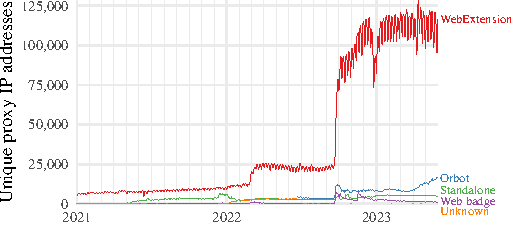
\includegraphics{figures/proxies/proxy-type}
\caption{
Unique proxy IP addresses per day,
by proxy type.
The two steps in the graph correspond
to the invasion of Ukraine by Russia in February~2022,
% 2022-02-25 https://twitter.com/torproject/status/1497276960556429324
% 2022-02-25 https://twitter.com/0xggus/status/1497224413829283877
and network restrictions in Iran beginning September~2022,
% 2022-09-24 https://twitter.com/torproject/status/1573670895696183303
% 2022-10-03 https://www.eff.org/deeplinks/2022/10/snowflake-makes-it-easy-anyone-fight-censorship
at which times there were campaigns
to encourage running Snowflake proxies.
Unknown proxy types (fewer than~50) are not shown.
}
\label{fig:proxy-type}
% 2021-02-23 https://github.com/guardianproject/orbot/releases/tag/16.4.1-BETA-2-tor.0.4.4.6
% "experimental mode to enable running as a Snowflake proxy"
% 2021-07-14 https://github.com/tladesignz/IPtProxy/commit/228e9e61e285ee548a42d6bee487577e44630695
% IPtProxy 1.1.0 changes its proxy type from "standalone" to "iptproxy"
% 2021-12-20 https://github.com/guardianproject/orbot/releases/tag/16.5.2-RC-1-tor.0.4.6.8
% Orbot updates IPtProxy from 1.0.0 to 1.2.0 https://github.com/guardianproject/orbot/commit/57add48cd904afe94363219887cd142bb5cf6696
% 2022-01-03 https://github.com/guardianproject/orbot/releases/tag/16.5.2-RC-5-tor.0.4.6.9
% This is close to the date (2022-01-05) when there's sudden growth in "Unknown",
% which is probably Orbot self-reporting as "iptproxy" and the broker throwing away that label for being unrecognized.
% 2022-03-21 https://gitlab.torproject.org/tpo/anti-censorship/pluggable-transports/snowflake/-/merge_requests/82
% Broker starts to recognize "iptproxy" as a probe type, but not deployed yet.
% 2022-05-03 https://github.com/tladesignz/IPtProxy/commit/c6ba25ef6ce8449476f734c626eadffdf55d0519
% IPtProxy 1.6.0 adds 'ProxyType: "iptproxy"' (no effective change, had already been done in a patch).
% 2022-06-21 https://bugs.torproject.org/tpo/anti-censorship/pluggable-transports/snowflake/40151
% Broker deployment, broker starts recording "iptproxy" in descriptors.
% 2022-07-05 https://github.com/guardianproject/orbot/releases/tag/16.6.2-RC-1-tor.0.4.7.8
% Orbot 16.6.2 RC 1 upgrades to IPtProxy 1.6.0.
% 2022-08-02 https://github.com/guardianproject/orbot/releases/tag/17.0.0-ALPHA-1-tor.0.4.7.8
% "updated UI based on new design spec: https://github.com/guardianproject/orbot/blob/NEW_UX/docs/design-spec-kindness-mode.md"
% "improved support for Snowflake Proxying "kindness" / volunteer mode"
% 2023-01-13 https://github.com/guardianproject/orbot/releases/tag/17.0.0-BETA-1-tor.0.4.7.11
% "easy access to Snowflake proxy 'kindness' mode"
\end{figure}

Snowflake's effectiveness depends on its proxies,
of~which there are several types.
The primary type is the web browser extension,
% "Creating a Snowflake WebExtension addon" https://bugs.torproject.org/tpo/anti-censorship/pluggable-transports/snowflake/23888
which, once installed, works in the background
while the browser is running.
There is also a ``web badge'' version of the proxy that does not require installation.
It~uses the same JavaScript code as the extension, but runs in an ordinary web page.
Some people leave a browser tab idling on the web badge page,
rather than install a browser extension.
Apart from the web-based proxies,
we~provide a standalone, command-line proxy
that does not require a browser.
% "Golang implementation of standalone snowflake proxy" https://github.com/keroserene/snowflake/pull/41
This version is convenient to install on a rented VPS, for example.
Running a long-term proxy at a fixed IP address
is somewhat at odds with Snowflake's goal of proxy address diversity and agility,
but these standalone proxies are valuable because
they tend to have less restrictive NATs,
making them compatible with more clients.
Finally, Orbot, a mobile app for accessing Tor,
besides being able to \emph{use} Snowflake for circumvention,
can also \emph{provide} Snowflake proxy service to others,
a~feature called ``kindness mode.''
% Only so called in Orbot v17+, which should be current by the time the paper is submitted.

\autoref{fig:proxy-type} shows the daily counts
of each proxy type.
Browser extension proxies predominate,
representing about 80\%
of 140,000 daily IP addresses.
% > library("tidyverse")
% > proxy_type <- read_csv("figures/proxies/proxy-type.csv", col_types = cols()) %>% filter("2023-10-01" <= date & date < "2023-10-15")
% > proxy_type %>% group_by(type) %>% summarize(unique_ips = sum(unique_ips)) %>% mutate(percent = 100 * unique_ips / sum(unique_ips)) %>% ungroup()
% # A tibble: 4 × 3
%   type       unique_ips percent
%   <chr>           <dbl>   <dbl>
% 1 badge          11484.   0.589
% 2 iptproxy      305017.  15.7
% 3 standalone     61100.   3.14
% 4 webext       1570862.  80.6
% > proxy_type %>% group_by(date) %>% summarize(unique_ips = sum(unique_ips)) %>% tail()
% # A tibble: 6 × 2
%   date       unique_ips
%   <date>          <dbl>
% 1 2023-10-09    143144.
% 2 2023-10-10    146650.
% 3 2023-10-11    147743.
% 4 2023-10-12    146602.
% 5 2023-10-13    141202.
% 6 2023-10-14    132032.
For comparison, there were about 1,900
of the more traditional style of Tor bridge at this time.
% https://metrics.torproject.org/networksize.csv?start=2023-10-01&end=2023-10-15
% date,relays,bridges
% 2023-10-12,8106,1859
% 2023-10-13,8012,1858
% 2023-10-14,8083,1862
The difference is attributable to the relative ease
of running a Snowflake proxy versus a Tor bridge---though
the comparison is not quite direct,
because Tor bridges have better defenses
against enumeration and blocking than do Snowflake proxies.

It~was not clear, at the outset,
that it would even be possible to attract
enough proxies to make Snowflake meaningfully blocking resistant
and support a reasonable number of users.
% "Start producing snowflakes" https://bugs.torproject.org/tpo/anti-censorship/pluggable-transports/snowflake/20813
Lowering the technical barriers to running a proxy was only part of~it;
getting there also took intentional advocacy and outreach.
In~the early days, circa~2017,
the only round-the-clock proxy support was
a few standalone proxies,
% 2018 "The three fallback proxy-go instances..." https://bugs.torproject.org/tpo/anti-censorship/pluggable-transports/snowflake/25688
run by us for the benefit of alpha tester clients.
The browser extension became available in mid-2019.
% |2019-06-26|||snowflake|Deployed version 0.0.1 of the Snowflake WebExtension for Firefox.|[comment](https://bugs.torproject.org/tpo/anti-censorship/pluggable-transports/snowflake/30931#note_2593598)||
% |2019-07-03|||snowflake|Deployed version 0.0.1 of the Snowflake WebExtension for Chrome.|[comment](https://bugs.torproject.org/tpo/anti-censorship/pluggable-transports/snowflake/30999#note_2593718)||
In~the latter half of 2019,
% |2019-07-26|||flashproxy snowflake|Cupcake 2.0 is released, now working with Snowflake rather than flash proxy.|[Chrome Web Store page](https://chrome.google.com/webstore/detail/cupcake/dajjbehmbnbppjkcnpdkaniapgdppdnc)||
% Cupcake stopped working when we changed the proxy–broker protocol:
% |2019-11-13 16:47:02|||snowflake|Restarted the broker with a new proxy–broker protocol.|[comment](https://gitlab.torproject.org/tpo/anti-censorship/pluggable-transports/snowflake/-/issues/29207#note_2592849)||
additional proxy capacity came when Cupcake,
a~browser extension for flash proxy with an existing user base,
was repurposed for Snowflake.
% "Link Cupcake from snowflake.torproject.org" https://bugs.torproject.org/tpo/anti-censorship/pluggable-transports/snowflake/31497
% "Snowflake integration" https://github.com/glamrock/cupcake/issues/24
Orbot's Snowflake proxy feature was added in version 16.4.1 in February~2021.
% https://github.com/guardianproject/orbot/releases/tag/16.4.1-BETA-2-tor.0.4.4.6 2021-02-23
% https://github.com/guardianproject/orbot/releases/tag/16.4.1-RC-1-tor.0.4.4.6 2021-04-09
% https://github.com/guardianproject/orbot/blob/a69f39bb37469e65730d0751519848ec29001959/CHANGELOG#L714 /** 16.4.1-RC-1 / 9 April 2021 / c80f18ae2508b73fcbfd6e09b394a2a196de7459 **/
% https://lists.mayfirst.org/pipermail/guardian-dev/2023-July/005708.html
% 16.4.1-BETA-2-tor.0.4.4.6 was released and promoted first, and had a visible effect on proxy counts,
% though 16.4.1-RC-1-tor.0.4.4.6 was the "real" 16.4.1 release.
(In~\autoref{fig:proxy-type}, Orbot is counted among the standalone proxies
until January~2022, when it got its own proxy type designation.)
% See history in figures/proxies/proxy-type.r.

It~is worth reflecting
on the greater popularity of the browser extension
compared to the web badge.
The latter had been envisioned
as the primary source of proxies in flash proxy,
% By the end of its run, flash proxy had also gained
% https://www.bamsoftware.com/talks/ee380-flashproxy/index.html#s15
% browser extensions including Cupcake
% "Chrome browser add-on" [Cupcake for flash proxy] https://bugs.torproject.org/legacy/trac/7721
% "Tor Flashproxy Badge" [for Firefox] https://github.com/reezer/tor-flashproxy-badge/
% and a standalone proxy.
% "Node.js standalone flash proxy" https://bugs.torproject.org/legacy/trac/7944
the idea being that people's browsers
would automatically become proxies
while reading sites that had the flash proxy badge installed,
unless they checked an option to prevent~it.
We~decided, early on, that flash proxy's opt-out permission had been a mistake,
% Date: Tue, 6 Dec 2016 18:38:40 -0800
% From: David Fifield <dcf@torproject.org>
% To: Arlo Breault <arlo@torproject.org>
% Cc: Serene <serene@torproject.org>
% Subject: Re: Snowing
% Message-ID: <20161207023840.mli4cymr6s3aanpu@happy.bamsoftware.com>
%
% My original plan was to repurpose existing flash proxy badges as
% Snowflake badges. But, I am thinking more and more that Snowflake should
% use an opt-in model, rather than opt-out. The opt-out model of flash
% proxy always bothered me. I think there's a good chance it would cause
% trouble for us if Snowflake becomes popular. So I'd like to see
% Snowflake use opt-in badges (and Cupcake) only.
and that Snowflake would be opt-in.
In~order to run a proxy, a person must take a positive action
such as installing a browser extension
or activating a toggle on a web page.
% "Prepare a Snowflake 'options' page, like in flashproxy" https://github.com/keroserene/snowflake/issues/21
Our initial worry that this policy
would reduce the number of proxies turned out to be unfounded.
People find an informative, interactive proxy control panel more appealing
than a nondescript badge graphic,
and install the browser extension in greater numbers
than ever used the web badge in flash proxy.

\subsection{Proxy churn}
\label{sec:proxy-churn}

% https://bugs.torproject.org/tpo/anti-censorship/pluggable-transports/snowflake/34075
% https://gitlab.torproject.org/tpo/anti-censorship/pluggable-transports/snowflake/-/merge_requests/95

The size of the proxy pool is not the only measure of its quality.
Also important is its ``churn,'' the rate at which
it is replenished with fresh proxy IP addresses.
Churn determines how hard a censor would have to work
to keep a blocklist of proxy IP addresses up to date;
or alternatively,
how quickly a momentarily complete blocklist
would lose effectiveness.

We ran an experiment to measure churn.
Every hour, the broker logged a record of
the proxy IP addresses it had seen in the past hour.
To~avoid storing real proxy IP addresses,
each record was not a transparent list,
but a HyperLogLog++ sketch~\cite{Heule2013a},
a~probabilistic data structure for estimating
the number of distinct elements in a multiset.
We~additionally hashed proxy IP addresses with a secret string
before adding them to a sketch,
to prevent their recovery from our published data.
A~sketch supports two basic operations: count and merge.
Given a sketch~\(X\),
we may compute an approximate count \(|X|\)
of its unique elements,
and given two sketches \(X\) and~\(Y\),
we~may merge them into a new sketch
representing the union \(X \cup Y\).
The quantity we are interested in,
the size of the intersection of two sketches,
is~computed using the formula
\(|X| + |Y| - |X \cup Y|\).
Such a computation estimates
how many IP addresses are shared across
two samples of the proxy pool.

\begin{figure}
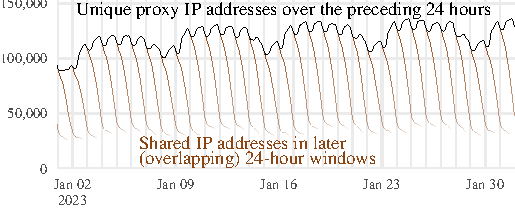
\includegraphics{figures/proxy-churn/proxy-count-decay}
\caption{
Proxy pool churn in January 2023.
The dark upper line shows the number
of unique proxy IP addresses in a 24-hour window
starting at the point indicated.
The lighter descending lines show
how many of the same IP addresses remain in the pool,
at 1-hour intervals up to 40 hours later.
It~takes about 20~hours for 50\% of the proxy pool to turn over.
}
\label{fig:proxy-count-decay}
\end{figure}

\autoref{fig:proxy-count-decay}
visualizes the results of the churn experiment.
We merged consecutive sketches over a 24-hour window
to serve as a reference,
then computed the size of its intersection
with other windows of the same size,
offset by \(+1, +2, \ldots, +40\) hours.
After 1~hour, the shifted window still has, on average,
97.3\% of addresses in common with the reference;
after 12~hours the fraction has fallen to 68.8\%;
by the time 24~hours have elapsed,
only 38.2\% of proxy IP addresses
are ones that had been seen in the previous day.
% > library("tidyverse")
% > options(width = 200)
% > DATE_RANGE <- as.Date(c("2023-01-01", "2023-02-01"))
% > read_csv("figures/proxy-churn/proxy-churn-windows.csv") %>%
%     filter(lubridate::`%within%`(reference_timestamp_end, do.call(lubridate::interval, as.list(DATE_RANGE)))) %>%
%     mutate(
%       sample_offset_hours = round(sample_timestamp_end_offset / 3600),
%       intersection_count = reference_count + sample_count - union_count
%     ) %>%
%     group_by(sample_offset_hours) %>%
%     summarize(
%       across(c(reference_count, sample_count, union_count, intersection_count), mean),
%       intersection_percent = 100 * intersection_count / reference_count,
%       .groups = "drop"
%     ) %>%
%     filter(sample_offset_hours %in% c(0, 1, 2, 3, 4, 8, 12, 18, 24, 36, 40))
% # A tibble: 11 x 6
%    sample_offset_hours reference_count sample_count union_count intersection_count intersection_percent
%                  <dbl>           <dbl>        <dbl>       <dbl>              <dbl>                <dbl>
%  1                   0         119654.      119654.     119654.            119654.                100
%  2                   1         119654.      119704.     122907.            116450.                 97.3
%  3                   2         119654.      119754.     126142.            113266.                 94.7
%  4                   3         119654.      119804.     129359.            110099.                 92.0
%  5                   4         119654.      119854.     132529.            106980.                 89.4
%  6                   8         119654.      120060.     145141.             94572.                 79.0
%  7                  12         119654.      120292.     157684.             82262.                 68.8
%  8                  18         119654.      120649.     176400.             63903.                 53.4
%  9                  24         119654.      120970.     194892.             45732.                 38.2
% 10                  36         119654.      121500.     206542.             34612.                 28.9
% 11                  40         119654.      121639.     208269.             33024.                 27.6

% \subsection{SQL injection attempts at broker}
% \url{https://bugs.torproject.org/tpo/anti-censorship/pluggable-transports/snowflake/40089}
% Actually tailored to the broker protocol, not a generic attack tool.

\section{Notable blocking attempts}
\label{sec:block}

In~\autoref{sec:clients} we saw how Snowflake's user counts
have at times been affected by the blocking actions of censors.
Now we take a closer look at selected censorship events.
The effect of censorship has usually been to increase rather than decrease
the number of Snowflake users.
This is no paradox:
as~censorship intensifies,
users are displaced from less resilient
to more resilient systems.
Snowflake's blocking resistance has not in every case been an unqualified success,
though, and here we also reflect on missteps
and persistent challenges.

The examples of this section are taken from
Russia, Iran, China, and Turkmenistan,
and are selected for being significant and instructive.
Common lessons are that lines of communication
and a good working relationship
with affected users are invaluable in quickly understanding and reacting to blocking;
and that blocking resistance
can only be understood in relation to a censor,
because every censor's cost calculus is different.

Snowflake is blockable by any censor that is willing to block WebRTC.
We~would not claim otherwise.
Indeed, we~believe this is how circumvention systems
should be presented:
not by arguing their unblockability in absolute terms,
but by laying out
what actions by the censor would suffice to block~it---or~more
to the point,
\emph{what sacrifices a censor would have to make}
in order to block~it.
Some censors may be able to make those sacrifices; others may not.
Advancing the state of the art of censorship circumvention
consists in pushing blocking
beyond the capabilities of more and more censors.

\subsection{Blocking in Russia}
\label{sec:block-ru}

% "[Russia] Some ISPs are blocking Tor" https://bugs.torproject.org/tpo/community/support/40050
% "OONI reports of Tor blocking in certain ISPs since 2021-12-01" https://ntc.party/t/ooni-reports-of-tor-blocking-in-certain-isps-since-2021-12-01/1477
% "Responding to Tor censorship in Russia" https://blog.torproject.org/tor-censorship-in-russia/
% "OONI shows blocking of Snowflake in select ISPs in Russia since 2023-02" https://ntc.party/t/ooni-shows-blocking-of-snowflake-in-select-isps-in-russia-since-2023-02

Snowflake, along with other common ways of accessing Tor,
was blocked in a subset of ISPs in Russia
% https://ntc.party/t/ooni-reports-of-tor-blocking-in-certain-isps-since-2021-12-01/1477/95
% "Tor filtering is done using government black box called TSPU.
% Not all providers have them. Tor is not blocked if TSPU is not present.
% According to tor metrics graph directly connecting users decreased only by 1/3.
% This indicates TSPU is not everywhere."
on \mbox{2021-12-01}~\cite{ooni-2021-russia-blocks-tor}.
The event was evidently coordinated and targeted,
as~it happened suddenly and affected multiple Tor-related protocols.
Besides Snowflake,
a~portion of Tor relays and bridges,
as~well as some servers of
the circumvention transports meek and obfs4,
were blocked, at~least temporarily.
As~might be expected, the attempt to block
various blocking-resistant protocols
was less than totally successful,
and its ultimate effect was to substantially increase the number
of users accessing Tor via circumvention transports,
Snowflake among them.
% "A zoom on just the bridge transports" https://bugs.torproject.org/tpo/community/support/40050#note_2796770
% That pluggable transports could not compensate fully
% for the loss of relay users points to a usability gap.

We~had the advantage of established relationships
with developers and users in Russia,
one of whom, through manual testing,
found the traffic feature that was being used to distinguish Snowflake.
It~was DTLS fingerprinting,
of~the kind cautioned about in \autoref{sec:fingerprinting}.
% "Russian DPI check supported_groups extension in ServerHello payload (byte 0x5a in udp packet)." https://bugs.torproject.org/tpo/anti-censorship/pluggable-transports/snowflake/40014#note_2765074
Specifically, it~was the presence of a
\mbox{supported\_groups} extension in the DTLS Server Hello message produced by Pion.
The extension being present in Server Hello was a bug in itself,
% "Server Hello should not contain supported_groups extension (extension.SupportedEllipticCurves)" https://github.com/pion/dtls/issues/409
but it also afforded the censor a feature to match on
that would detect DTLS connections with a Pion implementation in the server role,
without affecting other forms of DTLS.
The process of finding the flaw, fixing it,
and shipping new releases of Tor Browser took a few weeks,
% "Point to a forked version of pion/dtls with fingerprinting fix" https://gitlab.torproject.org/tpo/applications/tor-browser-build/-/merge_requests/375
% 2021-12-14 https://blog.torproject.org/new-release-tor-browser-115a1/
% 2021-12-20 https://blog.torproject.org/new-release-tor-browser-1103/
after which the user count rose quickly:
from the beginning to the end of December~2021,
the number of users in Russia grew from about 400 to about 4,000
% > library("tidyverse")
% > WANTED_FINGERPRINTS <- c(
%     "7659DA0F96B156C322FBFF3ACCC9B9DC01C27C73" = "snowman",
%     "5481936581E23D2D178105D44DB6915AB06BFB7F" = "snowflake-01",
%     "91DA221A149007D0FD9E5515F5786C3DD07E4BB0" = "snowflake-02"
%   )
% > userstats <- read_csv("figures/users/userstats-bridge-combined-multi.csv") %>%
%     filter(transport == "snowflake" & fingerprint %in% names(WANTED_FINGERPRINTS)) %>%
%     mutate(across(c(low, high), ~ .x / (coverage / pmax(num_instances, coverage)))) %>%
%     mutate(users = (low + high) / 2) %>%
%     # Combine the contributions of all bridges.
%     group_by(date, transport, country) %>% summarize(across(c(low, high, users), sum), .groups = "drop") %>%
%     # Apportion "??" to other countries (see figures/users/users-country.r).
%     group_by(date, transport) %>% mutate(across(c(low, high, users), ~ .x * sum(.x) / sum(ifelse(country == "??", 0, .x)))) %>% ungroup() %>% filter(country != "??")
% > userstats %>% filter(date %in% as.Date(c("2021-12-01", "2022-01-01"))) %>% filter(country == "ru")
% # A tibble: 2 x 6
%   date       transport country   low  high users
%   <date>     <chr>     <chr>   <dbl> <dbl> <dbl>
% 1 2021-12-01 snowflake ru       381.  381.  381.
% 2 2022-01-01 snowflake ru      4381. 4380. 4380.
(\autoref{fig:client-counts-ru}).
Snowflake was to become a significant tool
amid the general intensification of censorship in Russia
following the invasion of Ukraine in February~2022.

\begin{figure}
% Make the float take up an entire column.
% The \vphantom rule and \smash'ed minipage are because a plain minipage
% would count the depth of the descenders of the final line of text.
% See the TeXbook chapter 18, page 178.
% The output would otherwise look right, but yield a warning: Float too large for page by 2.18pt.
\vphantom{\rule{0pt}{\textheight}}\smash{%
\begin{minipage}[b][\textheight][b]{\linewidth}
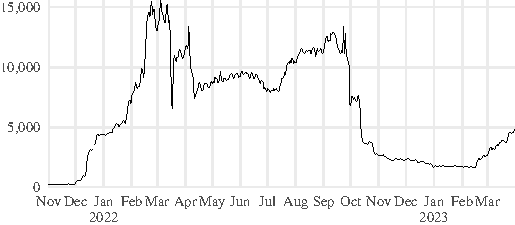
\includegraphics{figures/users/users-ru}
\caption{
Snowflake users in Russia (average concurrent).
The attempted blocking of Tor-related transports in December~2021
led to Snowflake's first surge in usage.
The decrease in September--October~2022
coincided with an even larger influx of users from Iran.
\label{fig:client-counts-ru}
}
\vfill
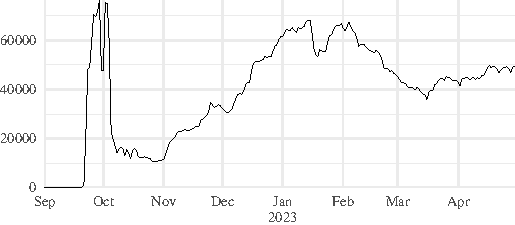
\includegraphics{figures/users/users-ir}
\caption{
Snowflake users in Iran.
Heightened censorship beginning in September 2022
caused Iran to become the single biggest source of Snowflake users.
The drop in October 2022
was the result of TLS fingerprint blocking,
which interfered with rendezvous
and took some time to mitigate.
\label{fig:client-counts-ir}
}
\vfill
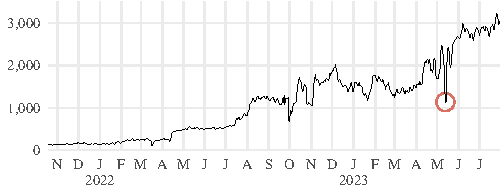
\includegraphics{figures/users/users-cn}
\caption{
Snowflake users in China.
Though no sustained blocking is evident,
disruption of domain fronting rendezvous
for three days in May 2023 briefly
depressed user numbers.
\label{fig:client-counts-cn}
}
\vfill
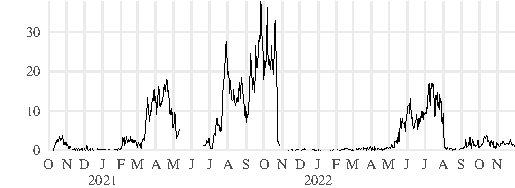
\includegraphics{figures/users/users-tm}
\caption{
Snowflake users in Turkmenistan.
Though there have never been many Snowflake users in Turkmenistan,
blocking events are evident on
% > library("tidyverse")
% > WANTED_FINGERPRINTS <- c(
%     "7659DA0F96B156C322FBFF3ACCC9B9DC01C27C73" = "snowman",
%     "5481936581E23D2D178105D44DB6915AB06BFB7F" = "snowflake-01",
%     "91DA221A149007D0FD9E5515F5786C3DD07E4BB0" = "snowflake-02"
%   )
% > userstats <- read_csv("figures/users/userstats-bridge-combined-multi.csv") %>%
%     filter(transport == "snowflake" & fingerprint %in% names(WANTED_FINGERPRINTS)) %>%
%     mutate(across(c(low, high), ~ .x / (coverage / pmax(num_instances, coverage)))) %>%
%     mutate(users = (low + high) / 2) %>%
%     # Combine the contributions of all bridges.
%     group_by(date, transport, country) %>% summarize(across(c(low, high, users), sum), .groups = "drop") %>%
%     # Apportion "??" to other countries (see figures/users/users-country.r).
%     group_by(date, transport) %>% mutate(across(c(low, high, users), ~ .x * sum(.x) / sum(ifelse(country == "??", 0, .x)))) %>% ungroup() %>% filter(country != "??") %>%
%     filter(country == "tm")
% > userstats %>% filter("2021-10-20" <= date & date <= "2021-10-28")
% > userstats %>% filter("2022-07-30" <= date & date <= "2022-08-07")
% # A tibble: 9 × 6
%   date       transport country   low  high users
%   <date>     <chr>     <chr>   <dbl> <dbl> <dbl>
% 1 2021-10-20 snowflake tm      33.0  33.1  33.0
% 2 2021-10-21 snowflake tm      27.3  27.8  27.5
% 3 2021-10-22 snowflake tm      23.1  23.6  23.4
% 4 2021-10-23 snowflake tm      18.9  19.5  19.2
% 5 2021-10-24 snowflake tm       5.56  6.19  5.87
% 6 2021-10-25 snowflake tm       1.63  2.23  1.93
% 7 2021-10-26 snowflake tm       2.12  2.64  2.38
% 8 2021-10-27 snowflake tm       1.29  1.40  1.35
% 9 2021-10-28 snowflake tm       1.05  1.72  1.39
% # A tibble: 9 × 6
%   date       transport country   low   high users
%   <date>     <chr>     <chr>   <dbl>  <dbl> <dbl>
% 1 2022-07-30 snowflake tm       6.29  7.92  7.11
% 2 2022-07-31 snowflake tm       5.66  7.76  6.71
% 3 2022-08-01 snowflake tm       8.43 10.6   9.51
% 4 2022-08-02 snowflake tm       3.03  5.25  4.14
% 5 2022-08-03 snowflake tm       0     1.47  0.735
% 6 2022-08-04 snowflake tm       0     1.24  0.618
% 7 2022-08-05 snowflake tm       0     1.32  0.659
% 8 2022-08-06 snowflake tm       0     0.619 0.310
% 9 2022-08-07 snowflake tm       0     0.771 0.386
\mbox{2021-10-24} and \mbox{2022-08-03}.
% \label is inside \caption so that the baseline of the last line
% of the caption aligns with the baseline of the other column.
% https://tex.stackexchange.com/a/298714
\label{fig:client-counts-tm}
}
\end{minipage}}
\end{figure}

The Server Hello \mbox{supported\_groups} distinguisher
used to detect Snowflake in Russia had been
discovered and documented by MacMillan et~al.~\cite[\S 3]{arxiv.2008.03254}
already in~2020.
We~might have avoided this blocking event by proactively fixing
the known distinguisher---but
it was not necessarily the wrong call not to have done~so.
In~a project like Snowflake,
there is always more to do than time to do~it;
one must consider the opportunity cost
of preempting specific blocking that may not come to pass.
In~this case, a~reactive approach by us was enough:
the loss was minor, and we were able to patch the problem quickly.
Even in the ISPs where the blocking rule was present,
it~did not succeed
at blocking 100\% of Snowflake connections,
because of the way it targeted a quirk of the Pion
implementation of Server Hello.
When the DTLS server role in the WebRTC data channel
was played by a web browser proxy,
not a standalone proxy or Snowflake client,
the feature would not be present.
% The Snowflake client would retry its rendezvous repeatedly,
% until hitting on a proxy that worked.

% "IRC Tip about Signature used to block Snowflake in Russia, 2022-May-16" https://bugs.torproject.org/tpo/anti-censorship/censorship-analysis/40030
% "Snowflake blocked by ClientHello [RU]" https://bugs.torproject.org/tpo/anti-censorship/pluggable-transports/snowflake/40140
% "A new Snowflake blocking rule (offset of supported_groups in DTLS Client Hello)" https://ntc.party/t/a-new-snowflake-blocking-rule-offset-of-supported-groups-in-dtls-client-hello/2420

In~May 2022 we got a report of a new detection rule,
this time keyed on not just the presence, but the \emph{contents}
of the \mbox{supported\_groups} extension,
now at a byte offset suggesting that
it targeted the Client Hello message,
not Server Hello.
The presence of a \mbox{supported\_groups} extension in Client Hello is not at all unusual,
but the specific groups offered by Pion's implementation
differed from those of common browsers.
Despite our being able to confirm the existence of the new blocking rule,
testers reported that Snowflake continued to work---which
% https://bugs.torproject.org/tpo/anti-censorship/censorship-analysis/40030#note_2804998
% https://ntc.party/t/a-new-snowflake-blocking-rule-offset-of-supported-groups-in-dtls-client-hello/2420/2
may have something to do with the fact that the Snowflake client
does not always play the client role in DTLS.
If~the Snowflake client is the DTLS server,
and the DTLS client is a browser proxy,
then the byte pattern looked for by the blocking rule does not appear.
% Hard to say at this point, but perhaps it was the cause of the sharp drop in April 2022, only reported in May?
We~developed a mitigation,
but by the time we had prepared a testing release in July~2022,
% "Creating a version of Tor Browser with patched Snowflake client that includes supported_groups censorship countermeasure" https://bugs.torproject.org/tpo/anti-censorship/team/83
% https://ntc.party/t/testing-invitation-for-tor-browser-with-supported-groups-patch-countermeasure-in-snowflake-to-evade-censorship-observed-in-russia/2837
the new rule
had apparently been removed
and replaced by another.
We~can only speculate as to motivations,
but it may be that the censor found the old rule
to have too many false positives,
or~simply not to be effective enough.

% "Блокировку Сlient Hello убрали, теперь блокируют Hello Verify Request" https://ntc.party/t/in-case-snowflake-rendezvous-gets-blocked/1857/9
% "They removed the blocking of Client Hello, now they block Hello Verify Request" https://bugs.torproject.org/tpo/anti-censorship/censorship-analysis/40030#note_2823140

The detection rule that replaced \mbox{supported\_groups} in Client Hello
looked for the presence of a Hello Verify Request message.
Hello Verify Request is an anti-denial-of-service feature in DTLS,
in~which the server sends a random cookie to the client,
and the client sends a second Client Hello message,
this one containing a copy of the cookie~\cite[\S 5.1]{rfc9147}.
Sending Hello Verify Request is not an error
(it~is a ``MAY'' in the RFC),
but because the Pion implementation in Snowflake sent~it,
and major browsers did not,
it was a reliable indicator of Snowflake connections.
(Those, at least, in which the DTLS server role was played by
a Snowflake client or standalone proxy.)
This distinguisher had also been anticipated by
MacMillan et~al.~\cite[\S 3]{arxiv.2008.03254} in~2020.
The first reports of this blocking rule were in July~2022;
but as you can see in \autoref{fig:client-counts-ru},
it~had no apparent immediate effect.
It~is hard to say whether the drastic decline in October 2022
was a consequence of this rule,
or some other, unidentified one.
That decline coincided with an explosion of users from Iran,
which temporarily affected the usability of the whole system.
We deployed a mitigation to remove the Hello Verify Request message
from Snowflake, regrettably, only in February~2023, % and only in Tor Browser, no Orbot yet
after which the number of users in Russia began to recover.
% "Apply Snowflake Remove HelloVerify Countermeasure" https://gitlab.torproject.org/tpo/applications/tor-browser-build/-/merge_requests/637
% "Since the release of Tor Browser 12.0.3 on 2023-02-15 there has been an increase in users from Russia on both bridges." https://bugs.torproject.org/tpo/anti-censorship/censorship-analysis/40030#note_2893870

The example of Snowflake in Russia
demonstrates some of the difficulty of censorship measurement.
The~answer to a question like ``Does Snowflake work in Russia?''
is not a simple yes or~no.
It~may depend on the date, the ISP,
and even such factors as which endpoint plays the DTLS server role.

\subsection{Blocking in Iran}
\label{sec:block-ir}

% "Unexplained drop in Snowflake client polls and bandwidth, testers wanted" https://github.com/net4people/bbs/issues/131
% "Tor censorship in Iran" https://bugs.torproject.org/tpo/anti-censorship/team/96#note_2840481
% "Sudden reduction in snowflake-01 bridge bandwidth, 2022-10-04 17:15" https://bugs.torproject.org/tpo/anti-censorship/pluggable-transports/snowflake/40207
% "Planning response to censorship in Iran with AC team" https://gitlab.torproject.org/tpo/team/-/wikis/Planning-response-to-censorship-in-Iran-with-AC-team

In~late September 2022,
users from Iran became the majority of Snowflake users almost overnight,
only to fall just as quickly two weeks later.
See \autoref{fig:client-counts-ir}.
The cause of the rise was
extraordinary new network restrictions amid mass protests~\cite{ooni-2022-iran-blocks-social-media-mahsa-amini-protests};
the cause of the decline was TLS fingerprint blocking,
which stopped Snowflake rendezvous from working.
Specifically, it~was a block of one of the TLS fingerprints
that may be used by the Snowflake client during rendezvous.

That simple TLS fingerprinting worked to block Snowflake rendezvous
was carelessness on our part.
Having anticipating such an event,
we~had already implemented TLS camouflage using uTLS
in the Snowflake client,
but failed to turn it on by default.
% "uTLS for broker negotiation" https://bugs.torproject.org/tpo/anti-censorship/pluggable-transports/snowflake/40054
Activating the feature required only a small configuration change,
% "Enable uTLS and use the full bridge line for snowflake" https://gitlab.torproject.org/tpo/applications/tor-browser-build/-/merge_requests/540
but we had to wait for new releases of Tor Browser and Orbot
to get it into the hands of users:
see the September--November~2022 interval in \autoref{fig:client-counts-ir}.

The fact that only one (albeit the most common)
of the Snowflake client's TLS fingerprints was blocked
could be a sign of carelessness on the part of the censor.
On~the other hand, it~is not certain that the TLS fingerprint blocking of October 2022
was meant to disrupt Snowflake specifically.
Go~is a popular language for implementing circumvention systems.
Snowflake may have been caught up in blocking that was intended for another system.

% "Blocking of cdn.sstatic.net by SNI in Iran, 2023-01-16 to 2023-01-24 and sporadically thereafter" https://bugs.torproject.org/tpo/anti-censorship/team/115#note_2873040

After repairing the TLS fingerprinting flaw,
the number of users from Iran gradually recovered
to near its former peak.
We~are aware of only minor disruptions after this time.
The default front domain used in rendezvous
was blocked (by~TLS SNI) in some ISPs
between \mbox{2023-01-16} and \mbox{2023-01-24}.
We~confirmed the block using data from the OONI
censorship measurement platform.
A~reduction in users is visible at this time.
AMP cache rendezvous was a successful workaround while the block was in effect.
After the block was lifted,
OONI measurements in the following weeks showed isolated cases
of failure to connect to the front domain.
These may have been further attempts at blocking.
If~they were, they did not have much of an effect.

\subsection{Blocking in China}
\label{sec:block-cn}

% "Investigate Snowflake blocking in China" https://bugs.torproject.org/tpo/anti-censorship/pluggable-transports/snowflake/32657

The user count graph from China,
\autoref{fig:client-counts-cn},
does not show any drastic changes
like others we have discussed so far.
There are a modest but respectable number of Snowflake users in China.
Though there have been no singular, sustained events,
we~have seen evidence of short-term or tentative
blocking of Snowflake in China.

In~May 2019, when Snowflake was still only in alpha release,
a~user in China reported a failure to connect.
Investigation revealed that the cause was IP address blocking of
the few Snowflake proxies that existed at the time.
% 2019-05-01 "I'm going to say that this a proxy blocking problem" https://bugs.torproject.org/tpo/anti-censorship/pluggable-transports/snowflake/30350#note_2593274
Rendezvous worked, and the STUN exchange worked,
but client and proxy could not establish a connection.
We~confirmed the evidence by temporarily running a new proxy
at a different IP address:
clients in China could connect when they happened to be assigned
that proxy by the broker.
This was back before the web browser extension proxy existed,
and the only consistent proxy support was standalone proxies
we developers ran ourselves at a static IP address.
This problem went away as the proxy pool grew in size.

Later that month, we discovered another form of blocking in China:
% 2019-05-15 "access to stun.l.google.com:19302 was blocked" https://bugs.torproject.org/tpo/anti-censorship/pluggable-transports/snowflake/30368#note_2593357
% 2019-05-17 "it looks like the initial connection to the default STUN server is being blocked" https://bugs.torproject.org/tpo/anti-censorship/pluggable-transports/snowflake/30350#note_2593299
that of the default STUN server,
of~which there was only one configured at the time.
% https://gitlab.torproject.org/tpo/applications/tor-browser-build/-/blob/4ff2be0b02e322716f06829e49c50f39795bf43c/projects/tor-browser/Bundle-Data/PTConfigs/linux/torrc-defaults-appendix#L5
The solution to this problem was to add more STUN servers
and select a subset of them to use on each rendezvous attempt.
% 2020-07-09 "Use STUN server compatible with RFC 5780 in proxy" https://gitlab.torproject.org/tpo/anti-censorship/pluggable-transports/snowflake/-/merge_requests/5
% 2020-07-23 "Choose a random subset from given STUN servers" https://gitlab.torproject.org/tpo/anti-censorship/pluggable-transports/snowflake/-/merge_requests/7
% 2020-07-10 "Update version of snowflake to allow the client to perform NAT discovery" https://gitlab.torproject.org/tpo/applications/tor-browser-build/-/merge_requests/11
% 2021-01-21 "As far as we know, setting new STUN servers unblocked Snowflake in China." https://bugs.torproject.org/tpo/anti-censorship/pluggable-transports/snowflake/30350#note_2723004
Curiously, it seems that when the STUN server was blocked,
the standalone proxies that had been blocked earlier that month became unblocked.
% 2019-05-27 "It seems once they blocked those stun servers, all snowflake bridges became reachable again." https://bugs.torproject.org/tpo/anti-censorship/pluggable-transports/snowflake/30368#note_2593360
% NB stun.l.google.com reported reachable (to ICMP at least) 2021-05-03: https://bugs.torproject.org/tpo/anti-censorship/pluggable-transports/snowflake/40044#note_2734125

% These were determined not to be GFW related, rather proxy bugs:
% 2019-08-25 "Hello, currently, in China, I can't open any webpage in 9.0a4 version Tor browser through snowflake bridge" https://bugs.torproject.org/tpo/anti-censorship/pluggable-transports/snowflake/31503
% 2019-09-22 "Hello, today after about two hours, I can't open any webpage in Tor browser through Snowflake bridge." https://bugs.torproject.org/tpo/anti-censorship/pluggable-transports/snowflake/31818
% 2019-10-02 "Hello, Currently, Tor Browser 9.0a7 can't connect to Tor network through Snowflake bridge." https://bugs.torproject.org/tpo/anti-censorship/pluggable-transports/snowflake/31930
% 2019-10-04 "Hello, currently, in China, Tor Browser 9.0a7 version can't establish a Tor network connection through snowflake bridge" https://bugs.torproject.org/tpo/anti-censorship/pluggable-transports/snowflake/31960
% 2019-12-01 "Yesterday, in China, I tried to connect to Tor network through snowflake bridge for 10 times. But all of the connections failed" https://bugs.torproject.org/tpo/anti-censorship/pluggable-transports/snowflake/32653
% 2019-12-21 "Hello, currently, in China, Tor Browser 9.5a3 still can't connect to Tor network through snowflake bridge." https://bugs.torproject.org/tpo/anti-censorship/pluggable-transports/snowflake/32833
% 2020-01-13 "Hello, currently, in China, Tor Browser 9.5a4 still can't connect to Tor network through snowflake bridge." https://bugs.torproject.org/tpo/anti-censorship/pluggable-transports/snowflake/32930

% Attributed to lack of Turbo Tunnel:
% 2019-11-25 "Hello, currently, in China, Tor Browser 9.5a2 still can't connect to Tor network through snowflake bridge" https://bugs.torproject.org/tpo/anti-censorship/pluggable-transports/snowflake/32597
% 2020-03-29 "Hello, currently, in China, Tor Browser 9.5a8 still can't connect to Tor network through snowflake bridge." https://bugs.torproject.org/tpo/anti-censorship/pluggable-transports/snowflake/33756

% Unresolved/needs information:
% 2021-05-03 "Hello, currently, in China, tor-browser-linux64-10.5a15 can not connect to Tor network through Snowflake bridge" https://bugs.torproject.org/tpo/anti-censorship/pluggable-transports/snowflake/40044

% "Confirmed block of default Snowflake in China" https://github.com/net4people/bbs/issues/249
% "Snowflake bridge does not work in China since days ago" https://forum.torproject.net/t/snowflake-bridge-does-not-work-in-china-since-days-ago/7635
% "Blocking of Snowflake in China, 2023-05-12" https://bugs.torproject.org/tpo/anti-censorship/censorship-analysis/40038
The next incidents we are aware of did not occur until 2023,
recent enough to be in the scope of \autoref{fig:client-counts-cn}.
On May~12, 13, and~14, a~few users reported problems
with domain fronting rendezvous.
We~could not get systematic measurements,
but some reports suggested that the blocking was triggered
by multiple (two or three) HTTPS connections
with the same TLS SNI to certain IP addresses within a short time.
It~is possible that Snowflake was not the main target of this
blocking behavior, and was affected only as a side effect.
If~it indeed had to do with Snowflake,
our best guess is that it was aimed at the multiple rendezvous
caused by the use of multiple bridges---though such a
policy would certainly also affect a large number of non-Snowflake connections.
The number of users from China was about halved during these three days.
On May~15, this blocking went away and user counts returned to normal.
% Reported at the same time, perhaps coincidental:
% "GFW at the Edge: Latest Development of China's Distributed Censorship System" https://github.com/net4people/bbs/issues/248

% Slowness, great bottleneck?
% "Analysis of speed deficiency of Snowflake in China, 2023 Q1" https://bugs.torproject.org/tpo/anti-censorship/pluggable-transports/snowflake/40251

\subsection{Blocking in Turkmenistan}
\label{sec:block-tm}

% "Blocking of Snowflake in Turkmenistan, 2021-10-24" https://bugs.torproject.org/tpo/anti-censorship/censorship-analysis/40024
% "On 2021-10-24, Snowflake users dropped drastically and thereafter went to zero." https://bugs.torproject.org/tpo/anti-censorship/censorship-analysis/40029#note_2787789

There have never been more than a few tens of Snowflake users in Turkmenistan.
Even so, it~has happened at least twice
that the number of users dropped suddenly to zero,
as~you can see in \autoref{fig:client-counts-tm}.
We~attributed the drops to multiple causes:
filtering of the default broker front domain
by DNS and TCP RST injection,
and blocking of certain UDP port numbers
commonly used by STUN.

Turkmenistan is a particularly challenging environment for circumvention.
Though unsophisticated, the censorship there
is more severe and indiscriminate
than in other places we have seen.
The fraction of the population that has access to the Internet is relatively small,
which makes it hard to communicate with volunteer testers
and lengthens testing cycles.
We~have been able to mitigate Snowflake blocking in Turkmenistan,
but only partly, and after protracted effort.

The drop on \mbox{2021-10-24} was caused by
blocking of the default broker front domain.
We~determined this by
taking advantage of a feature of the Turkmenistan firewall,
namely its bidirectionality.
% "I did some tests to see if it would be possible to measure blocking of SNI and DNS from outside Turkmenistan" https://bugs.torproject.org/tpo/anti-censorship/censorship-analysis/40029#note_2787781
% "Bidirectional DNS, HTTPS, HTTP injection in Turkmenistan" https://github.com/net4people/bbs/issues/80
Conveniently for analysis,
the firewall works in both directions:
packets that \emph{enter} the country are subject to injection
just as those that exit it are~\cite[\S 2]{Nourin2023a}.
By~sending probes into the country from outside,
we~found that the default broker front domain
was blocked at both the DNS and TLS layers.
% "...the block on Snowflake is effected by (at least) DNS and SNI blocking of the broker's front domain, cdn.sstatic.net." https://bugs.torproject.org/tpo/anti-censorship/censorship-analysis/40024#note_2767094
It~was some time---not until August 2022---before we got
confirmation from testers that an alternative front domain
worked to get around the block of the broker.
% 2022-08-18 "broker rendezvous peer received" https://bugs.torproject.org/tpo/anti-censorship/censorship-analysis/40024#note_2829121
% We~did not get confirmation whether AMP cache rendezvous also worked,
% % "it would be helpful to ask them to try the AMP cache rendezvous." https://bugs.torproject.org/tpo/anti-censorship/censorship-analysis/40024#note_2794947
% though our external testing indicated it would.
% % "www.google.com does not appear to be blocked" https://bugs.torproject.org/tpo/anti-censorship/censorship-analysis/40024#note_2767094

% This was not the only interference with Tor at the time.
% Five days later, on \mbox{2021-10-29}, Tor users not using circumvention transports
% dropped from about 1,000 almost to zero.
% https://bugs.torproject.org/tpo/anti-censorship/censorship-analysis/40029#note_2787789

The increase in the number of users from May to August 2022
visible in \autoref{fig:client-counts-tm} was caused by
a partial unblocking of the broker front domain on \mbox{2023-05-03}.
We~realized this only in retrospect,
by~looking at logs from Censored Planet~\cite{Raman2020c},
a~censorship measurement system that had continuous measurements
of the domain at that time, in~one autonomous system in Turkmenistan.
There was a clear shift from RST responses to successful TLS connections on that date.
DNS measurements are available only after that date,
so~they do not show a change, but they also showed no blocking.
The unblocking evidently permitted some users to connect as before.
But it must not have been nationwide, because as late as \mbox{2022-08-18},
some users reported that RST injection was still in place for them
(though DNS injection had ceased).
% 2022-08-18 "wsarecv: An existing connection was forcibly closed by the remote host." https://bugs.torproject.org/tpo/anti-censorship/censorship-analysis/40024#note_2829106

% Connection Assist
% July 2022
% https://gitlab.torproject.org/tpo/anti-censorship/rdsys/-/merge_requests/48

There was yet another layer to the blocking.
Even if they could contact the broker
(at~the default or an alternative front domain),
clients could not then establish a connection with a proxy.
% "...there's some progress in the sense that the broker connection is working now, but it looks like the client is having trouble connecting to the proxies." https://bugs.torproject.org/tpo/anti-censorship/censorship-analysis/40024#note_2829140
% "connection failed timeout waiting for DataChannel.OnOpen" https://bugs.torproject.org/tpo/anti-censorship/censorship-analysis/40024#note_2829121
Further testing revealed blocking of the default STUN port, UDP~3478.
% "And port 3478 is blocked in TM" https://bugs.torproject.org/tpo/anti-censorship/censorship-analysis/40024#note_2829127
A~client that cannot communicate with a STUN server
cannot find its own ICE candidate addresses (\autoref{sec:connection}),
which makes most WebRTC proxy connections fail.
(The exceptions are proxies without NAT and ingress filtering.
While there are some such proxies,
censorship in Turkmenistan also outright blocks
large swaths of the IP address space,
including data center address ranges where those proxies tend to run.)
% "Even if the user is unable to connect to any STUN servers and sends an SDP offer with no candidates, they should still be able to connect to proxies that are not behind a NAT or behind a full cone NAT" https://bugs.torproject.org/tpo/anti-censorship/censorship-analysis/40024#note_2889789
As~chance would have it, the NAT discovery feature we rely on
for testing the NAT type of clients requires
STUN servers to open a second, functionally equivalent listener
on a different port~\cite[\S 6]{rfc5780} (commonly port 3479).
Changing to those alternative STUN port numbers
let some users connect to Snowflake again.
% "this line... :3479... Works!" https://bugs.torproject.org/tpo/anti-censorship/censorship-analysis/40024#note_2829157
% 2022-08-25 "Use stun servers on port 3479 for turkmenistan" https://gitlab.torproject.org/tpo/anti-censorship/rdsys-admin/-/merge_requests/4
Specifically, STUN servers on port 3479 worked in AGTS,
one of two major affected ISPs.
The workaround did not work in Turkmentelecom, the other major ISP,
where port~3479 was blocked.
% "So the line where we switch to port 3479 only works for some people but not others?" https://bugs.torproject.org/tpo/anti-censorship/censorship-analysis/40024#note_2829235
Though we do not have continuous measurements to be sure,
we~suspect that the STUN port blocking began on \mbox{2022-08-03}
and precipitated the drop seen there in \autoref{fig:client-counts-tm}.
% OONI stunreachability measurements cease on 2023-07-31.
% https://explorer.ooni.org/search?since=2022-07-01&until=2022-10-31&failure=true&probe_cc=TM&test_name=stunreachability

The blocking techniques just described are crude,
surely resulting in significant overblocking---but
they nevertheless offer greater challenges to circumvention
than the more considered blocking of Russia and Iran.
We~highlight this to make the point that blocking resistance
cannot be defined in absolute terms,
but only in relation to a particular censor
and its predilections.
Censors differ not only in resources
(time, money, equipment, personnel),
but also in their tolerance
for the social and economic harms of overblocking.
Circumvention can only respond to and act within these constraints.
The government of Turkmenistan has evidently chosen
to prioritize political control
over a functioning network, to an extreme degree.
To paraphrase one of our collaborators:
``What they have in Turkmenistan can hardly be called an Internet.''
% https://bugs.torproject.org/tpo/anti-censorship/censorship-analysis/40024#note_2889792
In~a network already heavily damaged by oppressive policy,
the marginal harm caused by the clumsy blocking of
this or that circumvention system is relatively small.
This explains the sense in which a resource-poor censor
can ``afford'' certain blocking actions
that a richer, more capable censor cannot.

\section{Future work}
\label{sec:future}

A~natural extension of Snowflake would be
to have it access systems other than Tor---ordinary
VPNs, for example.
Tor has its benefits:
an~existing user base,
a~standard (pluggable transports) for integrating
circumvention modules,
and exit nodes separate from entry nodes,
which relieve the circumvention developer of the concerns associated
with actually exiting traffic to its destination.
But Tor has drawbacks as well,
notably its lower speed and
a~lack of support for UDP and other non-TCP protocols.
Nothing inherently ties Snowflake to Tor,
and it might easily be adapted to other systems.
One question is whether every Snowflake-like deployment
should manage its own pool of proxies,
or~if proxies can somehow be shared.
Building Snowflake's population of proxies
has been a substantial undertaking in itself---for
every project to have to repeat the process from scratch
would be a regrettable duplication of effort.
There is no reason why one proxy might not
serve multiple projects,
the client expressing its preference
in its rendezvous message.
But there would be design issues to work out.
While some proxy operators may be happy to donate
bandwidth to a free-to-use project like Tor,
they may need more incentive than altruism to help a commercial VPN.
A~shared deployment would impose additional friction on development
(making it harder to alter the proxy protocol, for example).
Rather than retrofit the current Tor-based proxies
with support for other systems,
a~next-generation proxy pool might be designed
from the ground up with multiple cooperating projects in mind.
If~it proved successful,
the Tor deployment could migrate to~it.

% "Multiplex - one client splits traffic across multiple proxies" https://bugs.torproject.org/tpo/anti-censorship/pluggable-transports/snowflake/25723
% "I'm thinking of 'striping' packets across multiple snowflake proxies simultaneously." https://lists.torproject.org/pipermail/anti-censorship-team/2020-February/000059.html
The Turbo Tunnel reliability layer of \autoref{sec:data-transfer}
was necessary for providing a continuous session abstraction
over a sequence of unreliable proxies.
But it might do even more:
in~particular, it should be possible
for a client to multiplex its traffic
over multiple proxies not just sequentially, but in parallel.
(Something like multipath~TCP.)
Sequence numbers in the inner reliability layer
would ensure a reliable stream, even when proxies
have different lifetimes and performance characteristics.
Multiplexing could increase performance by using the sum
of the bandwidths of the individual proxies,
and reduce variability by hedging against the
client being assigned one very slow proxy.
Using two or more proxies at once would
eliminate the brief pause for re-rendezvous
between consecutive proxies that now occurs.
Our experiments with multiplexing have so far
not shown enough benefit to justify the change,
though it may be a matter of tuning.
% "...the multiplexing patch in !11 makes no difference in throughput (and in some cases seems to make throughput worse)" https://bugs.torproject.org/tpo/anti-censorship/pluggable-transports/snowflake/25723#note_2718643
% "at least the multiplexed version is not slower than the regular version now" https://gitlab.torproject.org/tpo/anti-censorship/pluggable-transports/snowflake/-/merge_requests/11#note_2716658
And of course, analysis would be required
to determine whether simultaneous WebRTC connections
form a distinctive network fingerprint.

\section*{Availability}

This section has been anonymized for submission.
Here we will link to a web site and source code.
All of the programs of which Snowflake is composed are,
naturally, free software.
We will also link to the data and code needed to reproduce
the figures and calculations in this paper.

{
\raggedright
\bibliographystyle{snowflake}
\bibliography{snowflake}
}

\end{document}
